% 3_methodology.tex

\cleardoublepage
\chapter{Modelling of Launch System Dynamics}\label{chapter:Design}
% XXX Check this intro, as well as applicability statement, with Ingo


\textcolor{red}{This work aims to study the optimised trajectory and performance of a rocket-scramjet-rocket launch system, requiring the dynamics of a launcher to be modelled in some detail, based on a representative design.
	This chapter presents the design and modelling of a representative rocket-scramjet-rocket launch system, in which the scramjet stage is reusable for multiple launches. 
		This rocket-scramjet-rocket launch system is designed to launch small satellites to a 567km altitude sun-synchronous orbit and is based on the SPARTAN launch system concept, originally designed by Jazra, Preller \& Smart\cite{Preller2017b,Jazra2013}, and now being developed by The University of Queensland and Hypersonix.
		the SPARTAN launch system is used as the basis for a representative launch system within this study because it is the only rocket-scramjet-rocket launch system undergoing design, 
		 and it is up-to-date technologically because it is currently in the research and design process. In addition, the SPARTAN is relatively mature when compared to other small, multi-stage systems, with multiple studies dedicated to its design, which is based on the experimentally tested REST scramjet engines.   
	The rocket-scramjet-rocket launch system described in this chapter is used as a representative model for a partially-airbreathing, partially-reusable, three-stage small satellite launcher, and the optimal trajectory results and performance analysis produced are expected to be directly applicable to future iterations of the SPARTAN as well as generally applicable to other multi-stage airbreathing launch systems that use a 'space-plane' type design. }
	
	
	 %However, the designs of the airbreathing launchers studied in Section XXX do show some similarities, primarily due to the requirement for the airbreathing stages to fly within the atmosphere and return to land under aerodynamic control. The airbreathing launch systems that have been designed to date are all configured for sustained in-atmosphere flight, including large lifting surfaces and aerodynamic control capability. In addition to this, airbreathing launch systems must include the systems necessary for airbreathing operation and reusability, including thermal protection, engines, and any necessary auxiliary systems. 
	  %In general the 'space-plane' type design is utilised for airbreathing launch systems, including distinct wings on at least one stage, with aft control and stability surfaces. The complex design and numerous systems included within an airbreathing launch system mean that it is important to model each stage of a launcher accurately when determining its dynamics and performance. This is particularly true due to the importance of aerodynamic and engine performance to the efficiency of the launch system as a whole, owing to the large amount of time spent in-atmosphere. In order to understand the operation and performance of a small, multi-stage, airbreathing launch system, an accurate and detailed vehicle model must be used for trajectory modelling and optimisation. 
	  
	  %Because of the design complexity of airbreathing launch systems, and the relatively early stage of airbreathing launch system design, there is no one configuration of engine types and stages that can be considered 'typical' of an airbreathing launch system, and there is only one design of a rocket-scramjet-rocket system currently being investigated, as can be observed from the analysis of the currently existing airbreathing launch systems in Section XXX.}






\begin{figure}[ht]
	\centering
	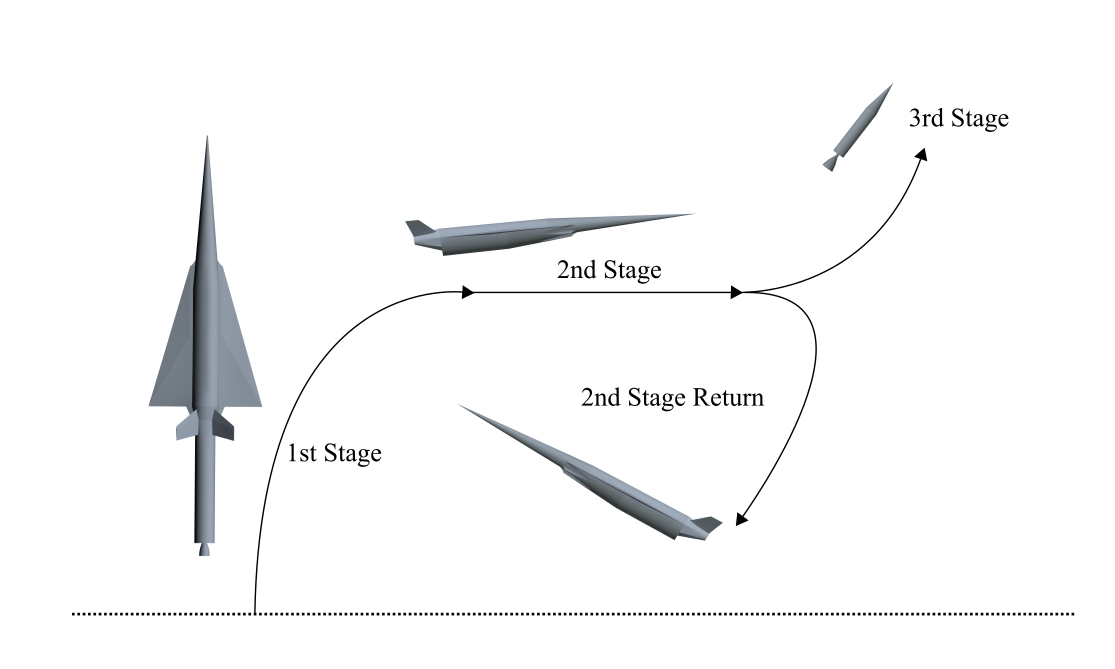
\includegraphics[width=0.9\linewidth]{figures/3_vehicle_design/Trajsimple}
	\caption{The launch process of the rocket-scramjet-rocket launch system, presented in simplified form.}
	\label{fig:Trajsimple}
\end{figure}



 Figure \ref{fig:Trajsimple} shows a simplified representation of the launch trajectory for the vehicle simulated in this study.
 The launch system is launched vertically under rocket power, from a traditional small rocket launch facility. The scramjet accelerator is mounted to the front of the first stage rocket allowing the scramjet accelerator to take the brunt of the aerodynamic forces and heating, as well as allowing the use of the control surfaces of the scramjet accelerator. During first stage rocket operation, the launch system pitches rapidly, reaching close to horizontal flight to allow the scramjet accelerator to stay at high dynamic pressure conditions. The scramjet accelerator is accelerated to its minimum operating velocity of approximately Mach 5, at which point separation occurs. The scramjet accelerator's four scramjet engines are ignited, and the scramjet accelerator is accelerated through the atmosphere, reaching approximately Mach 9. At this point, the specific impulse of the scramjet engines, and thus the efficiency of the scramjet accelerator, have decreased, and the third stage rocket is separated. The third stage rocket accelerates and performs a pull-up, before cutting its engine and coasting out of the atmosphere. Once the rocket is exoatmospheric, the engine is reignited, performing first a circularisation burn, and then a Hohmann transfer to the intended orbit. Meanwhile, the scramjet accelerator banks and executes a fly-back manoeuvre to return to its initial launch site. The scramjet accelerator extends landing gear, and lands on a traditional runway in the style of a conventional aircraft. The scramjet accelerator is able to be rapidly refurbished and remounted for further launches. To fulfil the requirements of this trajectory, the scramjet accelerator must be able to fly and manoeuvre from velocities greater than Mach 9 to landing, as well as being able to withstand high structural and heating loads without significant deterioration.
 
 The launch configuration of the SPARTAN is shown in Figures \ref{fig:NoInternal} \& \ref{fig:INTERNALS}. 
 The size and external design of the scramjet accelerator are used exactly as defined for the Baseline vehicle designed by Preller \& Smart\cite{Preller2017b}. Both the first and third stage rockets are designed in this study, and are sized around the Baseline vehicle. 
 The first stage rocket has not previously been designed, and as such is created for this study, while the third stage is redesigned to use a SpaceX Kestrel engine. This third stage design replaces the third stage used in previous SPARTAN studies, which was powered by a Pratt \& Whitney RL-10-3A engine\cite{Preller2017b}. The pump-fed RL-10-3A engine was deemed too costly, and it has been replaced by a significantly cheaper pressure-fed Kestrel engine in this study.  
 The internal layout of the scramjet accelerator has been reconfigured around this redesigned third stage. 
 This launch system weighs a total of \textcolor{red}{28355}kg, and is 32.44m long. 
 
 The following sections present the detailed design of the launch system, along with the aerodynamic and propulsion modelling of each stage.
The scramjet accelerator design is presented first, as the design of the scramjet accelerator drives the operational requirements and sizing of the launch system, and thus the design of the first and third stage rockets. 


\begin{figure}[ht]
	\centering
	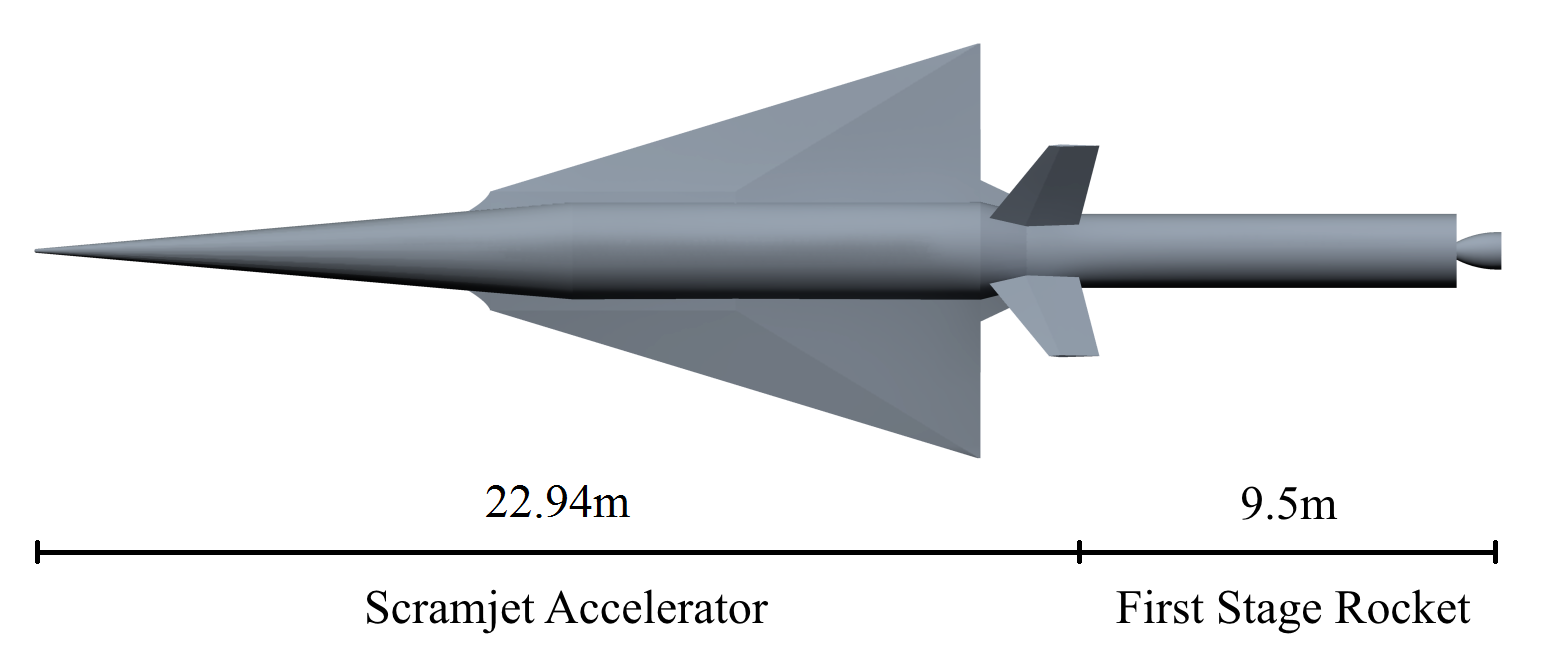
\includegraphics[width=0.7\linewidth]{figures/3_vehicle_design/NoInternal}
	\caption{The SPARTAN launch system, top view, showing the scramjet accelerator and first stage. }
	\label{fig:NoInternal}
\end{figure}

\begin{figure}[ht]
	\centering
	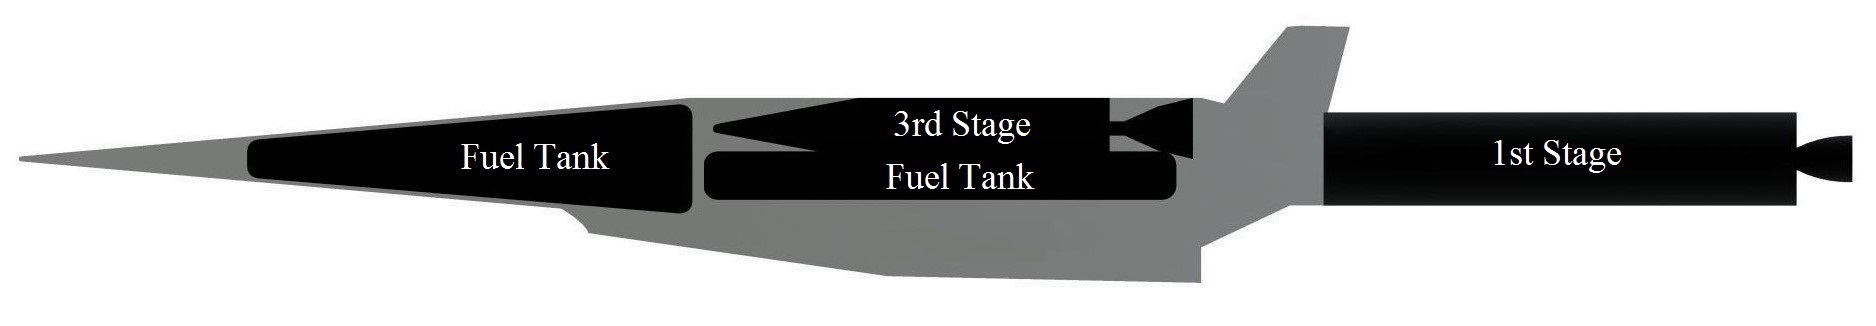
\includegraphics[width=0.7\linewidth]{figures/3_vehicle_design/INTERNALS}
	\caption{The SPARTAN launch system, side view, showing the scramjet accelerator and fuel tanks, along with the third and first stages. }
	\label{fig:INTERNALS}
\end{figure}









	
	
	\section{The Second Stage Scramjet Accelerator}\label{sec:SPARTAN}
 
		\subsection{The Scramjet Accelerator}
		
		The \textcolor{red}{representative scramjet-powered accelerator vehicle used in this study}, shown in Figure \ref{fig:SPARTANlabelled}, is based closely on the Baseline vehicle designed by Preller \& Smart\cite{Preller2017b}. \textcolor{red}{The external geometry of the scramjet accelerator is unchanged in this study, and is used to provide a baseline scale to the launch system.} The scramjet accelerator is 22.94m long, with a frontal cone half angle of 5$^\circ$\cite{Preller2017b}. 
		\begin{figure}[ht]
			\centering
			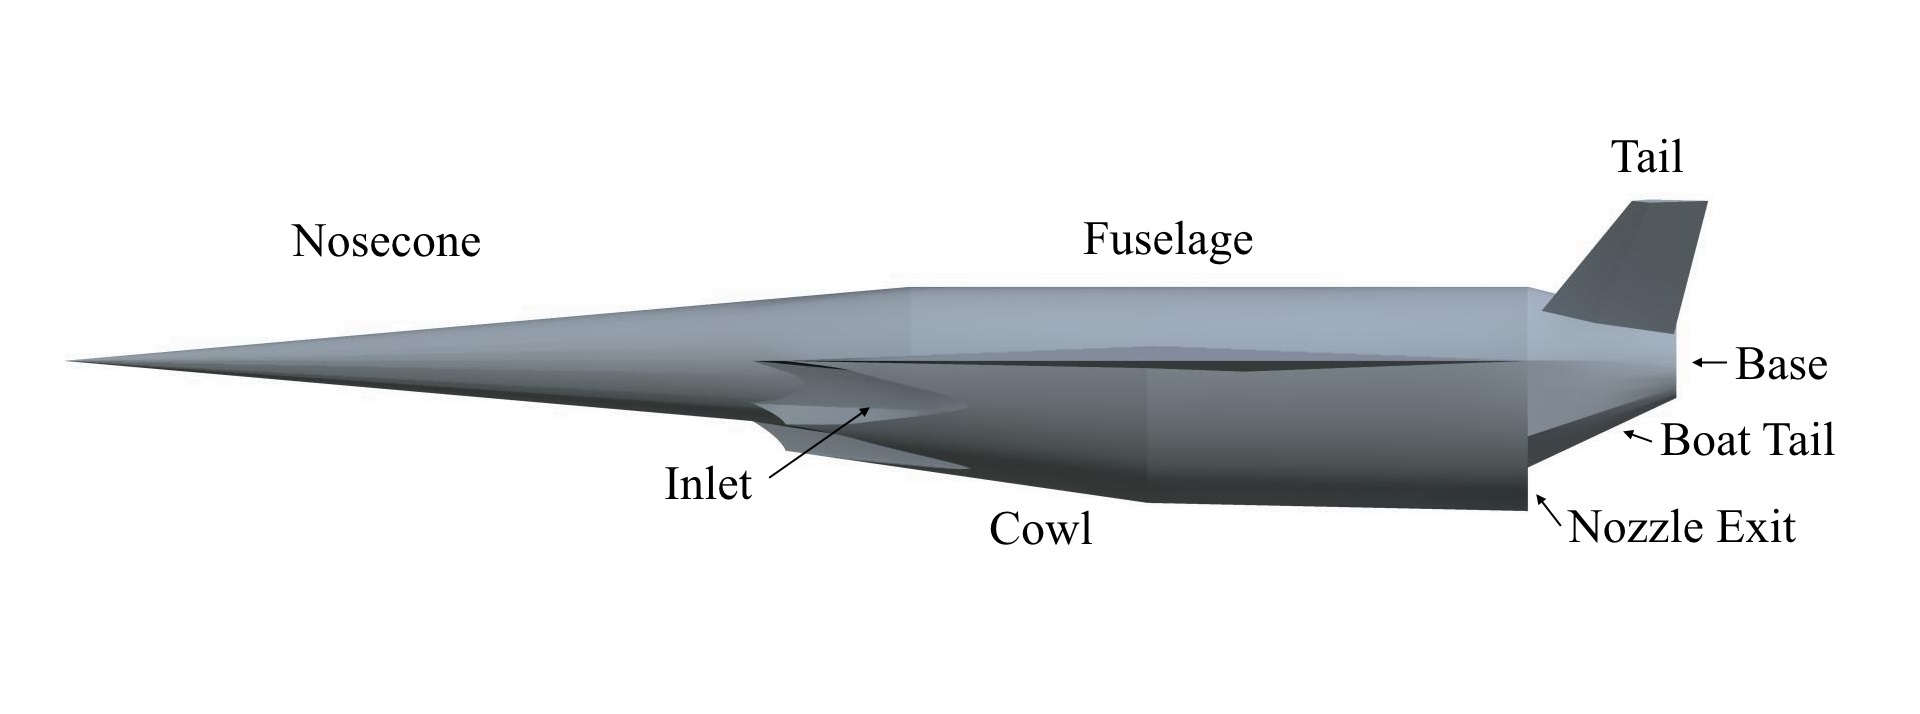
\includegraphics[width=0.7\linewidth]{figures/3_vehicle_design/SPARTANlabelled}
			\caption{The external features of the scramjet accelerator.}
			\label{fig:SPARTANlabelled}
		\end{figure}
		A mass breakdown of the scramjet accelerator is shown in Table \ref{tab:MassBreakdown}, adapted from previous work by Preller \& Smart\cite{Preller2017b}. \textcolor{red}{The fuel mass of the scramjet accelerator has been modified for the representative launch system in this work, as} the fuel tank sizes and total fuel mass are sized to accommodate the Kestrel-powered third stage, described in Section \ref{sec:ThirdStageBaseline}.
		\begin{table}[h]
		\begin{tabular}{|c|c|c|c|c|c|c|c|c|}
			\hline  \textbf{Part} & Total & Fuselage & Wings & Tanks & Systems & Landing Gear & Scramjets & Fuel \\ 
			\hline \textbf{Mass} (kg) & 6519.1 & 2861.6 & 350.7 & 179.4 & 707.5 & 188.9 & 669.0 & 1562.0 \\ 
			\hline 
		\end{tabular} 
		\caption{Mass breakdown of the modified scramjet accelerator vehicle.}
		\label{tab:MassBreakdown}
		\end{table}
This study assumes that the third stage is stored within the fuselage of the scramjet accelerator for simplicity. It is assumed that the release mechanism for the third stage is able to be situated within the available space surrounding the third stage, however the release mechanism is not considered further in this study \textcolor{red}{(see Section XXX)}. %- modelling uncertainties and simplifications)}
		
		
		% LH2 density
		 %http://webbook.nist.gov/cgi/fluid.cgi?Action=Load&ID=C1333740&Type=SatT&Digits=5&PLow=.5&PHigh=1.5&PInc=.1&RefState=DEF&TUnit=K&PUnit=atm&DUnit=kg/m3&HUnit=kJ/mol&WUnit=m/s&VisUnit=uPa*s&STUnit=N/m%

		The fuel tanks are sized to fit around the kestrel-powered third stage. There are three fuel tanks; two cylindrical tanks situated underneath the third stage; and a truncated conical tank in the nose. The conical fuel tank is designed to fit immediately forward of the third stage. This fuel tank is 8m long, leaving 1.47m$^3$ of space in the nose for cooling systems, frontal landing gear, and any additional systems or sensors which are necessary in the nose cone. The cylindrical tanks are positioned underneath and slightly to either side of the third stage, leaving space underneath for vehicle systems. The cylindrical fuel tanks are designed to be 8.5m long, with diameters of 0.87m, sized to give a nominal total tank volume of 22m$^3$.
The resized fuel tanks hold a total of 1562kg of LH2 fuel. This assumes an LH2 density of 71kg/m$^3$, slightly denser than LH2 at phase transition point at 1 atm.
The mass of the fuel tanks is scaled, by surface area, from Dawid Preller's Baseline vehicle model\cite{Preller2017b}, giving a total fuel tank mass of 179.4kg.
		
		\textcolor{red}{
			\subsection{Thermal Protection}
				}
			%- I need to frame this as a reference vehicle based on the SPARTAN
			%-it is assumed that thye SPARTAN will be capable of flying at const q, as in previous studies
			%-SPARTAN has tungsten tip
			%-It is acknowledged that the current TPS is likely to require the addition of active cooling, for the leading edges of the scramjet and the control surfaces, as well as the combustor
			%-mention yielding limit at high temps
			%-mention dlrs transpiration cooling and heat transport to eliminate local hot spots such as in scott kasens thesis?
		%	-this is currently a project proposal by darpa http://thermalsummit.com/2018/12/darpa-to-host-hypersonic-thermal-management-material-design-program/
		%	-I should cite something that says where max heating is, and the studies which show analyses of the stagnation points
		%	-\cite{Marley2017} is a good paper
	
		%-multilayer insulation is designed for operation at 1000 degrees C
		%-differentiate between heating at stagnation points (which are probably not connected directly to multilayer %insulation) and points around the vehicle which are likely to be connected directly
		%ie. stagnation points are calculated to see if the TPS will hold other points are calculated to see if 1000C is exceeded on insulated side 

The scramjet accelerator is thermally protected by a 11.3mm thick Carbon-Carbon aeroshell, with an alumina-borosilicate mat/ stainless steel multilayer insulator at the connection points between the aeroshell and the aluminium internal structure\cite{Preller2018a}. The nose tip of the scramjet accelerator is protected by 40mm thick tungsten, weighing 92kg, to provide rapid heat dissipation and sink in the area of greatest heating. For the purposes of this work it is assumed that the external shell is not connected to the internal structure close to points of large heating such as leading edges, and is structurally independent in these regions. 
In previous studies, a similar heat shielding has been assumed to provide adequate protection for the scramjet accelerator flying along a constant dynamic pressure trajectory\cite{Preller2018a}, and this assumption is used in the main body of this work. The thermal properties of the launch system are investigated further in Section \textcolor{red}{XXX} and it is concluded that a more advanced thermal protection system may be necessary. However, the full redesign of the thermal protection system of the SPARTAN is beyond the scope of this report, particularly as this is currently an area of significant research effort, and there are many possibly viable options for the cooling of hypersonic systems. 

\subsection{Propulsion}\label{sec:propulsion}

The scramjet accelerator is powered by four underslung scramjet engines, fuelled by liquid hydrogen. These engines are Rectangular To Elliptical Shape Transition (REST) engines, configured to allow for a conical forebody (C-REST). REST engines have a rectangular to elliptical shape transition inlet, and an elliptical combustor, offering simplicity in design as well as reduced thermal loading and viscous drag compared to scramjets with planar geometries\cite{Suraweera2009}.  REST engines are also specifically designed to operate over a wide range of Mach numbers, and at off design conditions, making them particularly applicable to use on scramjet accelerator vehicles. 


\subsubsection{Propulsion Modelling}\label{sec:Propulsion}


\textcolor{red}{
\begin{figure}
	\centering
	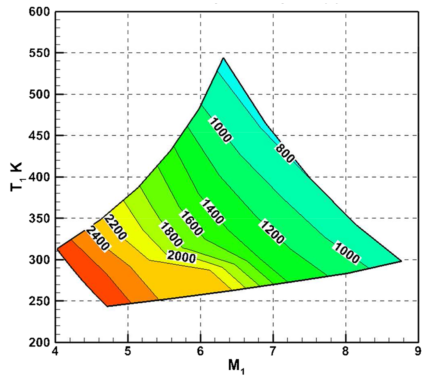
\includegraphics[width=0.7\linewidth]{figures/2_literature-review/C-REST}
	\caption{The C-RESTM10 propulsion database, specific impulse.}
	\label{fig:C-REST}
\end{figure}
To deliver a payload to orbit, the SPARTAN's scramjet accelerator stage uses four Rectangular-to-Elliptical Shape Transition (REST) scramjet engines, with inlets configured to allow installation on a conical forebody (C-REST). The C-REST engines that the scramjet accelerator uses have been configured to fly between Mach 5 and 10. This type of engine is known as a C-RESTM10 engine\cite{Preller2017b}. The REST engine has been shown experimentally to operate successfully at off design conditions\cite{Smart2006,Smart2009a}, and has shown good agreements with numerical CFD models\cite{Smart2009a}. 
}
\textcolor{red}{
A C-RESTM10 propulsion database has been used in previous studies to model the scramjet engines of the scramjet accelerator\cite{Preller2017b}. The specific impulse profile of the C-RESTM10 engine, taken from the C-RESTM10 propulsion database, is shown in Figure \ref{fig:C-REST}. This database has been created through separate modelling of the compression within the inlet, combustion within the combustor, and expansion through the internal nozzle\cite{Preller2018a}. The inlet compression was modelled by performance curves based on a set of CFD solutions\cite{Preller2018a}. These performance curves are used to obtain the flow conditions at the end of the inlet. The combustor is modelled using quasi-one-dimentional cycle analysis, assuming a combustion efficiency of 80\%\cite{Preller2018a}. Lastly, the properties at the end of the combustor are expanded assuming a nozzle efficiency of 90\%\cite{Preller2018a}.
The C-RESTM10 is designed for operation at M$_0$ = 10, and the contraction ratio and combustor divergence are not optimal for operation at low Mach numbers. At low Mach numbers, an equivalence ratio of 1 may cause the flow to choke and unstart. 
Consequently, an equivalence ratio of less than 1 was set at low Mach numbers, in order to avoid unstart\cite{Preller2018a}. At these Mach numbers, the C-REST engines are operating in dual-mode\cite{Preller2018a}. 
}
% Above moved from lit review 

 The C-REST engines are simulated separately to the aerodynamic simulations of the scramjet accelerator, using a combination of quasi-1D flow path analysis and performance curves based on high fidelity CFD simulations\cite{Preller2017b,Preller2018a}. The engine model takes the conditions at the inlet, and calculates the exit conditions and propulsive properties of the engine. The engine exit conditions are added into the aerodynamic simulations and the propulsive properties are used in the simulated vehicle model.
\begin{figure}[ht]
	\centering
	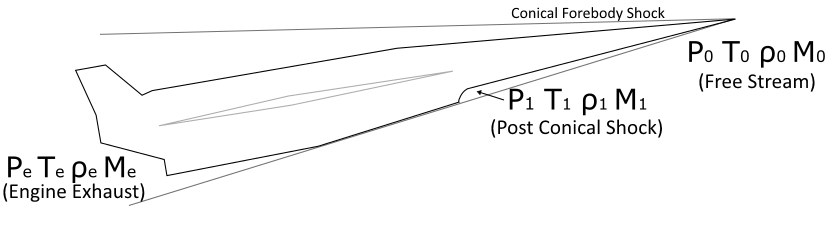
\includegraphics[width=0.7\linewidth]{figures/3_vehicle_design/SPARTANEngineshock}
	\caption{The locations of conditions relevant to C-REST engine simulation. }
	\label{fig:SPARTANEngineshock}
\end{figure}

\begin{figure}[ht]
	\begin{subfigure}{.5\textwidth}
		\centering
		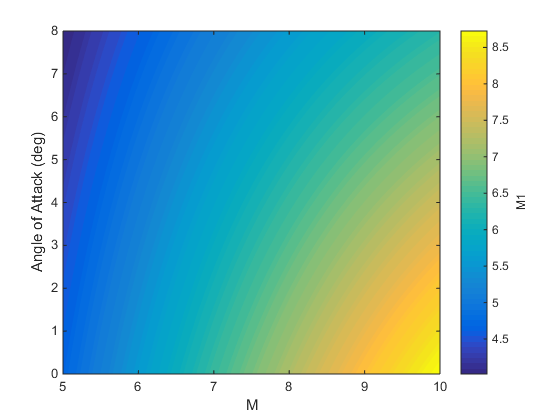
\includegraphics[width=0.99\linewidth]{figures/3_vehicle_design/ConicalM}
		\caption{Mach number.}
		\label{fig:ConicalM}
	\end{subfigure}
	\begin{subfigure}{.5\textwidth}
		\centering
		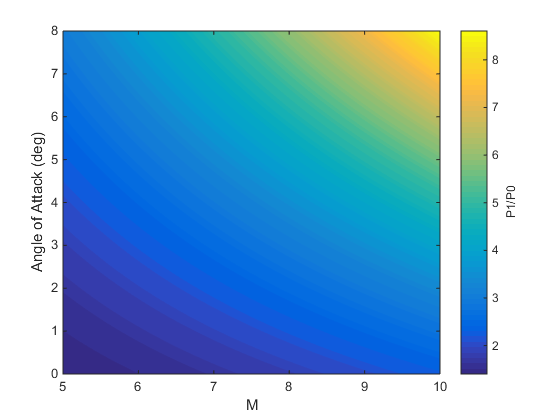
\includegraphics[width=0.99\linewidth]{figures/3_vehicle_design/ConicalP}
		\caption{Pressure ratio.}
		\label{fig:ConicalP}
	\end{subfigure}
	\begin{subfigure}{.5\textwidth}
		\centering
		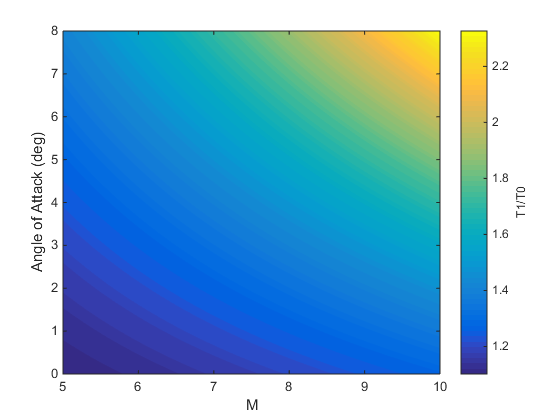
\includegraphics[width=0.99\linewidth]{figures/3_vehicle_design/ConicalT}
		\caption{Temperature ratio.}
		\label{fig:ConicalT}
	\end{subfigure}
	\caption{Flow conditions after the conical shock generated by the vehicle nose cone as a function of flight Mach number and angle of attack. Figure a) shows the Mach number, b) shows the pressure ratio, and c) shows the temperature ratio following the conical shock, at the engine inlet.}
	\label{fig:ConicalShock}
\end{figure}
Before the flow enters the engine, it is affected by the conical shock generated by the forebody of the scramjet accelerator.
Figure \ref{fig:SPARTANEngineshock} shows the locations of the flow properties, which are necessary to calculate engine performance. The ambient atmospheric conditions are calculated by interpolation using the 1976 NASA Atmospheric properties\cite{Administration1976}.
The flow properties at the inlet of the engines is calculated using the Taylor-Maccoll analysis method for conical shocks\cite{TaylorMaccoll}. This calculation is performed in the \textsf{cone\_shoot} program provided for this study by Prof. Michael Smart. The flow conditions as a function of flight conditions following the conical shock are shown in Figure \ref{fig:ConicalShock}.  





 The engine model used is based on the \textsf{CRESTM10} database\cite{Preller2017b,Preller2018a}, analysed using quasi-1D simulation and provided for this study by Prof. Michael Smart. This database has previously been used in simulations of the scramjet accelerator, as detailed in Section \textcolor{red}{XXX}.
This database provides data points of engine performance over inlet conditions within the operational range, at 50kPa dynamic pressure equivalent conditions. The specific impulse data set is shown in Figure \ref{fig:ISPinterp}. This data is interpolated for the given inlet conditions, to calculate specific impulse produced by the engine. As the data points of the \textsf{CRESTM10} database are unevenly distributed for inlet Mach and temperature, care must be taken in order to interpolate smoothly to allow the optimal control solver to converge successfully. To ensure that smooth interpolation is achieved, the \textsf{CRESTM10} database is first interpolated using linear interpolation, for each `set' of four nodes which form a square. A uniform grid is created using this linear interpolation, on which a cubic spline interpolation is applied using Matlab's \textsf{griddedInterpolant} function. This is explained in detail in Appendix \ref{Appendix:sim}. During flight the C-REST inlet conditions generally stay within the region bounded by the available data. However, for the purposes of the trajectory optimisation, it is necessary to provide data for a wide range of inlet conditions (T$_1$, M$_1$). To calculate $I_{SP}$ and equivalence ratios outside of the modelled range of inlet conditions, the existing data is extrapolated. This extrapolation is performed in the same manner as the interpolation, a linear extrapolation, followed by a cubic spline interpolation of the extrapolated points. This allows for smooth continuity between the interpolated and extrapolated points, while ensuring that the extrapolated regions provide reasonable values. 

For operation at high Mach numbers, the fuel mass flow rate is assumed to be stoichiometric, so that $\dot{m_f}$ = $0.0291\dot{m}$. This ensures that the scramjet engines are performing at high efficiency throughout the acceleration of the scramjet stage. 
\begin{figure}[ht]
	\centering
	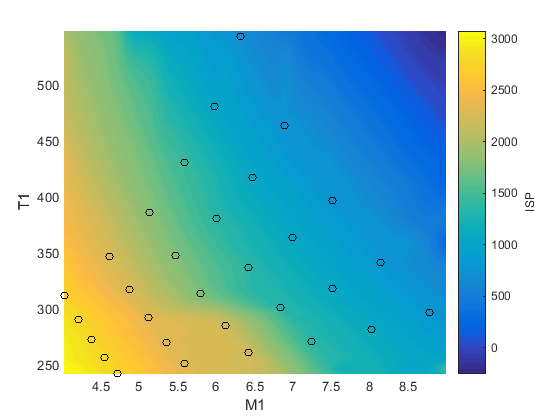
\includegraphics[width=0.6\linewidth]{figures/3_vehicle_design/ISPinterp}
	\caption{Specific impulse of the C-REST engines with input temperature and Mach number. Available data points are indicated.}
	\label{fig:ISPinterp}
\end{figure}
However, the C-REST engine is a fixed geometry engine, primarily designed for operability at high Mach numbers\cite{Preller2017b}. At lower Mach numbers, the addition of excessive fuel may cause the engine to choke and unstart, resulting in total loss of thrust\cite{Preller2017b}. To avoid unstart, an equivalence ratio ($\phi$) of less than 1 is necessary at low Mach numbers. In this region the equivalence ratio is set to the maximum value which does not cause the engine to unstart. The equivalence ratio interpolation is linear, as the number of data points available for interpolation is low. The prescribed equivalence ratio over the range of scramjet engine operation is shown in Figure \ref{fig:EquivalenceRatioInterp}.
\begin{figure}[ht]
	\centering
	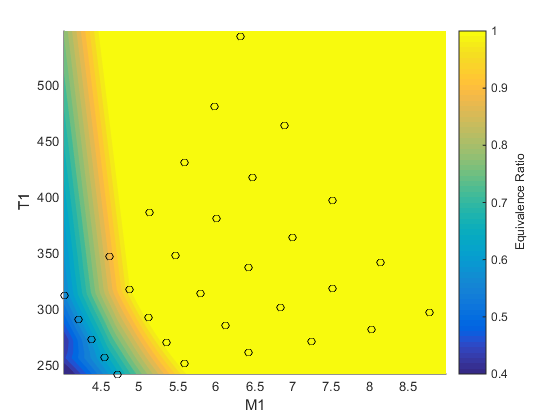
\includegraphics[width=0.6\linewidth]{figures/3_vehicle_design/EquivalenceRatioInterp}
	\caption{Operable equivalence ratio of the C-REST engines with input temperature and Mach number. Available data points are indicated.}
	\label{fig:EquivalenceRatioInterp}
\end{figure}
For these conditions, the fuel mass flow rate is determined by approximating the flow into the inlet as an ideal gas; 
\begin{equation}
\dot{m} = 0.9 m_c A_{cap} P_0 M_0 \sqrt{\dfrac{\gamma_0}{R_{air} T_0}},
\end{equation}
\begin{equation}
\dot{m}_{fuel} = (\dfrac{m_{fuel}}{m_{ox}} )_{st} \phi \dot{m}.
\end{equation}
The multiplier of 0.9 is an approximate term included to account for losses due to asymmetry within the engine\cite{Preller2018a}. 
The thrust for each engine, $T$, is obtained by inclusion of the interpolated specific impulse, ie. 
\begin{equation}
T = g_0\dot{m}I_{sp}. 
\end{equation}

In the available database, the C-REST engine was modelled to a nozzle exit area of 0.5586m$^2$. This is smaller than the exit area modelled on the version of the scramjet accelerator used in this work, of 0.9719m$^2$. For this reason, additional thrust is obtained from an additional nozzle segment, and the specific impulse of the C-REST engines will be higher than calculated in the database. The modelling of this additional nozzle segment and the thrust obtained are detailed in Section \ref{sec:engine-oncart}.






		
		
		\subsection{Aerodynamics}\label{sec:aero}
		
		
		
In order for the trajectory of the SPARTAN to be successfully simulated and optimised, the aerodynamics of the scramjet accelerator must be calculated for the large range of flight conditions experienced during its acceleration and return flights. 
The aerodynamics of the scramjet accelerator are calculated at set flight conditions covering the breadth of necessary conditions, and the results are tabulated in databases. During trajectory simulations, the aerodynamics of the scramjet accelerator are determined by interpolation over the aerodynamic databases using bivariate splines, and the drag and lift produced are calculated using the standard definition of the aerodynamic coefficients:

\begin{equation}
F_d = \frac{1}{2}\rho C_D v^2 A ,
\end{equation}

\begin{equation}
F_L = \frac{1}{2}\rho C_L v^2 A .
\end{equation}


\begin{figure}[ht]
	\centering
	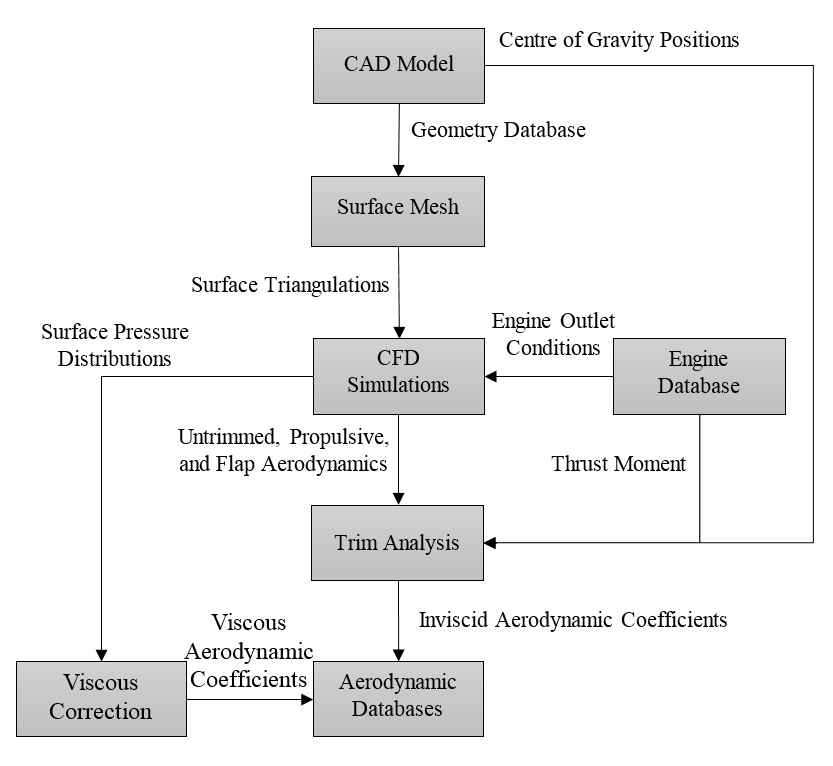
\includegraphics[width=0.7\linewidth]{figures/3_vehicle_design/FlowChart}
	\caption{The process for generating aerodynamic databases.}
	\label{fig:FlowChart}
\end{figure}

The trimmed aerodynamic databases of the scramjet accelerator are generated in full prior to trajectory simulation to improve the computational efficiency of the simulation. The aerodynamic coefficients of lift, drag and moment are tabulated, and these tables are interpolated during simulation. 
The aerodynamics are calculated for Mach numbers between 0-10, angles of attack between 0$^\circ$ and 10$^\circ$, and for altitudes between 0-40km. Separate aerodynamic simulations are performed for engine-on and engine-off conditions, as the operation of the scramjet engines changes the aerodynamic characteristics of the scramjet accelerator significantly. When the engines are powered-on, the engines are generating thrust on the internal nozzle, as well as on the boat tail and base.  When the scramjet engines are not operational air flows through the engine flowpath without fuel injection, generating a large amount of drag. 


The process for generating the aerodynamic databases is shown in Figure \ref{fig:FlowChart}. First, a CAD model of the scramjet accelerator is developed, providing the centre of gravity of the scramjet accelerator, as well as a geometry database which is used to create triangulated surface meshes. These surface meshes are then imported into the inviscid CFD solver Cart3D\cite{CART3D}, which calculates flow solutions to determine the aerodynamics of the scramjet accelerator at various flight conditions. CFD solutions are generated for the scramjet accelerator with the scramjet engines turned off, with the scramjet engines operational, and for a range of flap deflections. 
The flap deflections necessary to trim the vehicle are calculated at every flight condition, by balancing the aerodynamic moment of the scramjet accelerator with the aerodynamic moment generated by the flaps. 
The additional lift and drag generated by the flaps are then added to the untrimmed aerodynamics to create a trimmed database.
Finally, the viscous components of the aerodynamics of the scramjet accelerator are calculated, and added to the aerodynamic database. These processes are described in detail in the following sections. 







\subsubsection{Cart3D Simulations}\label{sec:cart3d}


\begin{figure}[ht]
	\centering
	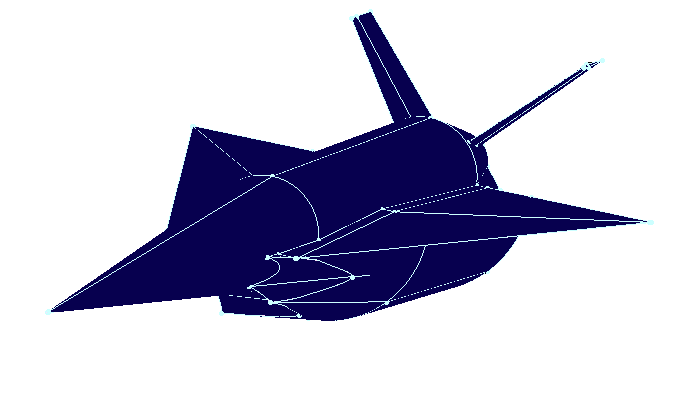
\includegraphics[width=0.6\linewidth]{figures/3_vehicle_design/Pointwise}
	\caption{Surface triangulation of the scramjet accelerator, generated using Pointwise\cite{Pointwise}.}
	\label{fig:Pointwise}
\end{figure}

The aerodynamics of the SPARTAN have been calculated using Cart3D, an inviscid CFD package used in the preliminary design of aerospace vehicles. Cart3D utilises adjoint mesh adaption with a Cartesian cut-cells approach to produce an iteratively refined mesh to fit a flow solution. Cart3D is used to generate the aerodynamic database of the SPARTAN due to its applicability in both the subsonic
and supersonic regimes, and its robustness across multiple flow solutions\cite{Sagerman2017,Abeynayake,Aftosmis2011,Almosnino2016a,Gomez2004}. Cart3D has previously been used to
analyse hypersonic vehicles, and has shown good agreement with experimental data across multiple studies\cite{Sagerman2017,Abeynayake,Aftosmis2011,Almosnino2016a}, as described in Section \ref{sec:Cart3d}.


\begin{figure}[ht]
	\begin{subfigure}{.5\textwidth}
		\centering
		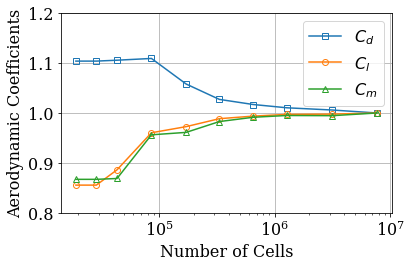
\includegraphics[width=0.99\linewidth]{figures/3_vehicle_design/CartCoeffs_cells}
		\caption{}
	\end{subfigure}
	\begin{subfigure}{.5\textwidth}
		\centering
		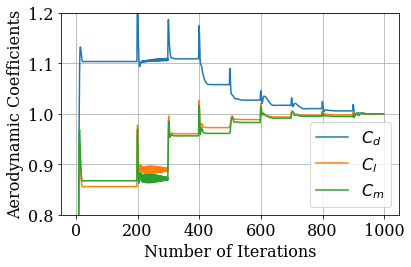
\includegraphics[width=0.99\linewidth]{figures/3_vehicle_design/CartCoeffs_its}
		\caption{}
		
	\end{subfigure}
	\begin{subfigure}{.5\textwidth}
		\centering
		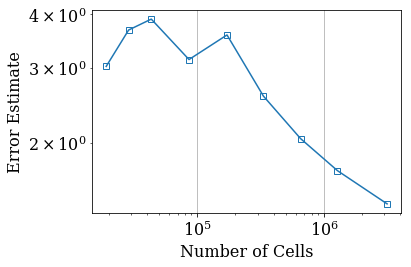
\includegraphics[width=0.9\linewidth]{figures/3_vehicle_design/ErrorEst}
		\caption{}
		
	\end{subfigure}
	
	\caption{The convergence of a Cart3D simulation of the scramjet accelerator at Mach 6, 2$^\circ$ angle of attack.}
	\label{fig:Cart3dValidation}
\end{figure}

Initially, a surface triangulation of the scramjet accelerator is created in Pointwise, shown in Figure \ref{fig:Pointwise}. This is then imported into CART3D as a watertight surface. 
The Cart3D Meshes are then initiated with an outer boundary distance of 40 times the vehicle length. This boundary distance has been observed to produce suitable free stream conditions and good mesh convergence. Nine mesh adaption levels are used. Nine levels have been observed to generally produce good convergence, with moderate computation times of 1-3 hours per simulation. The convergence of the residuals and forces are investigated to ascertain if a solution has converged. Figure \ref{fig:Cart3dValidation} shows an example solution validation for Mach 6, 2$^\circ$ angle of attack, engine-on conditions. Good convergence can be observed in the force functionals, with a corresponding decrease in the error estimate of the functional indicating solution convergence.  

Following simulation in CART3D over the required flight conditions, the aerodynamic coefficients are extracted. The simulation files are processed using Clic, a subprogram of CART3D used to calculate aerodynamic forces and moments, given surface pressure distributions. 
For engine-off aerodynamics, the aerodynamic coefficients of the entire scramjet accelerator are extracted. However, for the engine-on aerodynamics of the scramjet accelerator, the engine flowpath, boat tail and base of the scramjet accelerator are removed when the aerodynamic coefficients are extracted. The flowpath of the scramjet engines is assumed to be replaced by the conditions given by the \textsf{CRESTM10} engine database, and a separate Cart3D simulation is used to calculate the aerodynamic forces on the boat tail and base. 



\subsubsection{Engine-On Aerodynamic Analysis}\label{sec:engine-oncart}

When the scramjet engines are turned on, the exhaust exits the nozzle of the engines and expands onto the boat tail of the scramjet accelerator. This changes the aerodynamics of the boat tail significantly, necessitating separate Cart3D simulations to calculate the varied aerodynamic coefficients of the boat tail. In addition, 
the scaled engine modelled in the \textsf{CRESTM10} propulsion analysis has an exit area of 0.5586m$^2$, smaller than the nozzle exit area on the scramjet accelerator, of 0.9719m$^2$. The larger nozzle exit of the scramjet accelerator provides additional expansion area, and additional thrust, which must be modelled using Cart3D. 

The exhaust of the C-REST engines is simulated using CART3D, using SurfBC boundary conditions, which produce outflow and intflow conditions at the inlet and exit of the scramjet engines\cite{Pandya2004}. The exit conditions calculated by the \textsf{CRESTM10} database, as defined in Section \ref{sec:Propulsion}, are set as the inflow conditions for the Cart3D surface. 
The inflow surfaces are positioned inside the nozzle on the scramjet accelerator model, scaled to match the exit area of the engines simulated for the \textsf{CRESTM10} database, 0.5586m$^2$. The surface triangulation of the scramjet accelerator with outflow surfaces is shown in Figure \ref{fig:Pointwise-EngineBC}.
\begin{figure}[ht]
	\centering
	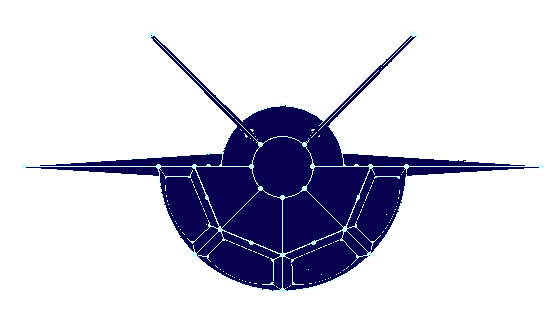
\includegraphics[width=0.7\linewidth]{figures/3_vehicle_design/Pointwise-EngineBC}
	\caption{View of the scramjet accelerator surface triangulation showing engine outlet boundaries.}
	\label{fig:Pointwise-EngineBC}
\end{figure}
Cart3D performs simulations nondimensionally, and requires the outflow conditions of a boundary to be normalised. The outflow conditions of $P_e$, $\rho_e$ and $M_e$ given by the \textsf{CRESTM10 }propulsion model are normalised to Cart3D nondimensionalised variables as follows\cite{Cartplumes,Mehta2015};

\begin{equation}
P_e^* = P_e/(\gamma_0 P_0),
\end{equation}

\begin{equation}
\rho_e^* = \rho_e/\rho_0,
\end{equation}

\begin{equation}
M_e^* = \sqrt{\gamma_e/\gamma_0 (M_e \sqrt{ P_e^*/\rho_e^*})^2}.
\end{equation}
Where $^*$ indicates the nondimensionalised input to Cart3D. This nondimensionalisation includes a correction on the Mach number to account for variation in the specific heat ratio, which is not possible to include directly in Cart3D\cite{Mehta2016}. The exhaust of the scramjet engines expands through the additional area of the scramjet accelerator's nozzle, and is further expanded onto the boat tail on the rear of the scramjet accelerator fuselage. This expansion causes significant force on the boat tail of the scramjet accelerator, generating additional lift, thrust, and moment forces. The total thrust generated by the scramjet accelerator, including the thrust generated by the additional nozzle expansion, and the forces on the boat tail, are shown in Figure \ref{fig:Thrust}, with the corresponding specific impulse shown in Figure \ref{fig:Isp}.



\begin{figure}[ht]
	\centering
	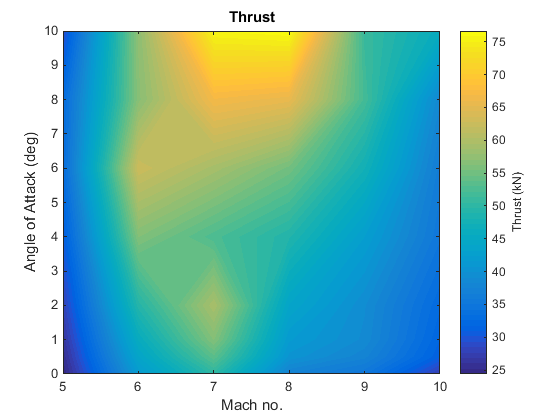
\includegraphics[width=0.6\linewidth]{figures/3_vehicle_design/Thrust}
	\caption{The total thrust output of the scramjet accelerator, including the CRESTM10 database, and Cart3D nozzle and boat tail simulations.}
	\label{fig:Thrust}
\end{figure}

\begin{figure}[ht]
	\centering
	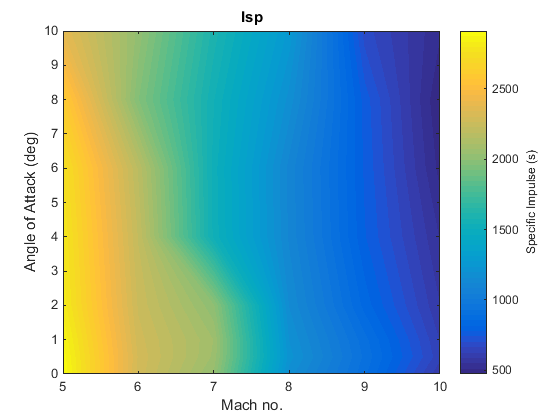
\includegraphics[width=0.6\linewidth]{figures/3_vehicle_design/Isp}
	\caption{The specific impulse of the scramjet accelerator, including the C-rest database, and Cart3D nozzle and boat tail simulations.}
	\label{fig:Isp}
\end{figure}


		
		
		
		
		
		
		\subsubsection{Centre of Gravity Analysis}
		The centre of gravity locations of the SPARTAN are calculated using CREO. For simplicity, it is assumed that structural, systems and landing gear masses are homogeneously distributed throughout the centre fuselage of the scramjet accelerator. 
		The calculated centre of gravity for the scramjet accelerator full of fuel and including the third stage rocket is \textcolor{red}{15.24m} along the body length. The centre of gravity varies as fuel is depleted throughout the acceleration phase, and at third stage release, changing the flap deflections required for trim. The cylindrical fuel tanks are depleted first, in order to shift the centre of gravity forward, and improve the aerodynamic stability of the scramjet accelerator during the majority of flight. Depleting fuel from the cylindrical fuel tanks first would likely also serve to reduce fuel slosh during flight, although the fuel slosh is not modelled in this study, and it is assumed that the centre of gravity of each individual tank remains constant. After the cylindrical tanks have been depleted, the fuel in the conical tank within the nose is used. The third stage is released at the end of acceleration, and the centre of gravity changes significantly. When the third stage is released there is still fuel stored in the conical tank for flyback, during which centre of gravity change must also be modelled. 
		Consequently, aerodynamic databases are created for centre of gravity conditions of; 
		\begin{itemize}
			\item full of fuel including third stage,
			\item conical fuel tank full of fuel, including third stage,
			\item empty of fuel including third stage,
			\item conical fuel tank full of fuel after third stage release,
			\item and empty of fuel after third stage release.
		\end{itemize}
		Each of these conditions, along with the corresponding centre of gravity, is shown in Figure \ref{fig:CentreOfGravity}. At each of the listed centre of gravity conditions, aerodynamic coefficients and flap deflections necessary for trim are calculated.  As each fuel tank is depleted, and the centre of gravity shifts, the aerodynamics at the two closest centre of gravity conditions are interpolated to produce the aerodynamics of the scramjet accelerator.  
		
		
		\begin{figure}
			\begin{subfigure}{.5\textwidth}
				\centering
				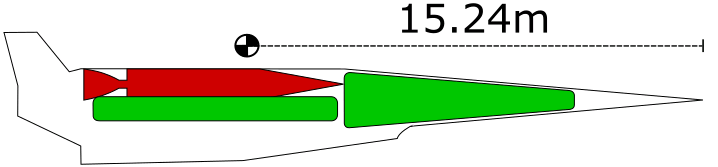
\includegraphics[width=0.9\linewidth]{figures/3_vehicle_design/CG1}
				\caption{Full of fuel, before third stage release.}
			\end{subfigure}
			\begin{subfigure}{.5\textwidth}
				\centering
				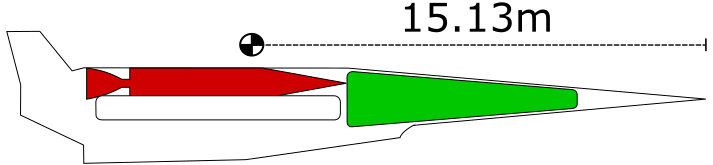
\includegraphics[width=0.9\linewidth]{figures/3_vehicle_design/CG2}
				\caption{Conical fuel tank full, before third stage release.}
				
			\end{subfigure}
			\begin{subfigure}{.5\textwidth}
				\centering
				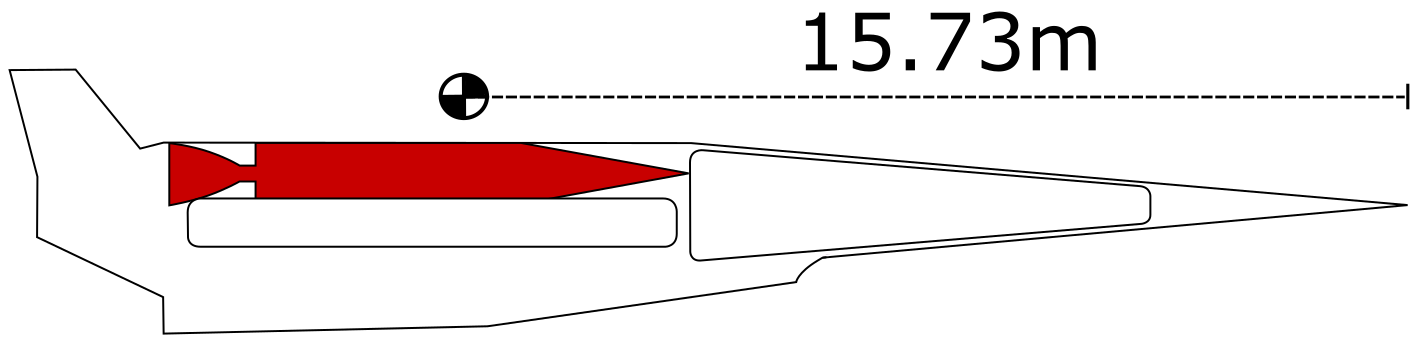
\includegraphics[width=0.9\linewidth]{figures/3_vehicle_design/CG3}
				\caption{Empty of fuel, before third stage release.}
				
			\end{subfigure}
			\begin{subfigure}{.5\textwidth}
				\centering
				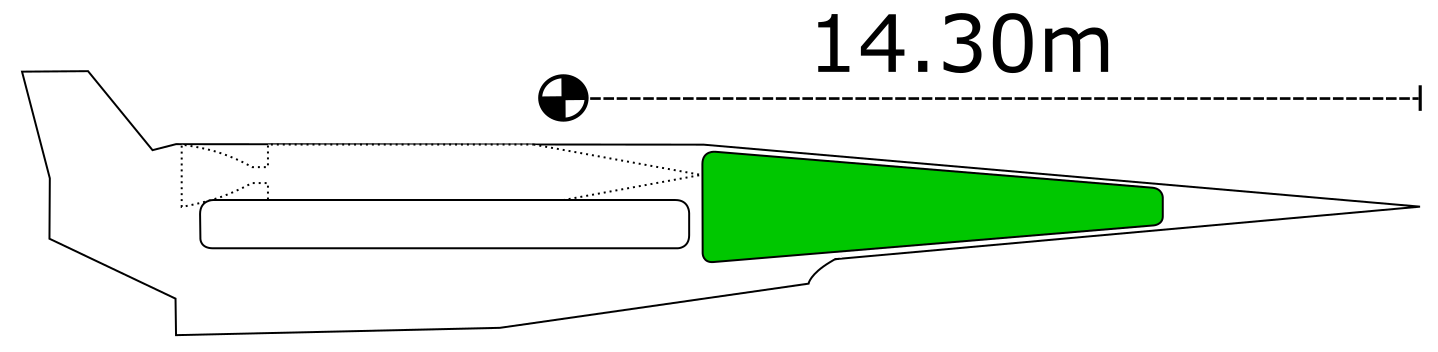
\includegraphics[width=0.9\linewidth]{figures/3_vehicle_design/CG4}
				\caption{Conical fuel tank full, after third stage release, engines off.}
				
			\end{subfigure}
			\begin{subfigure}{.5\textwidth}
				\centering
				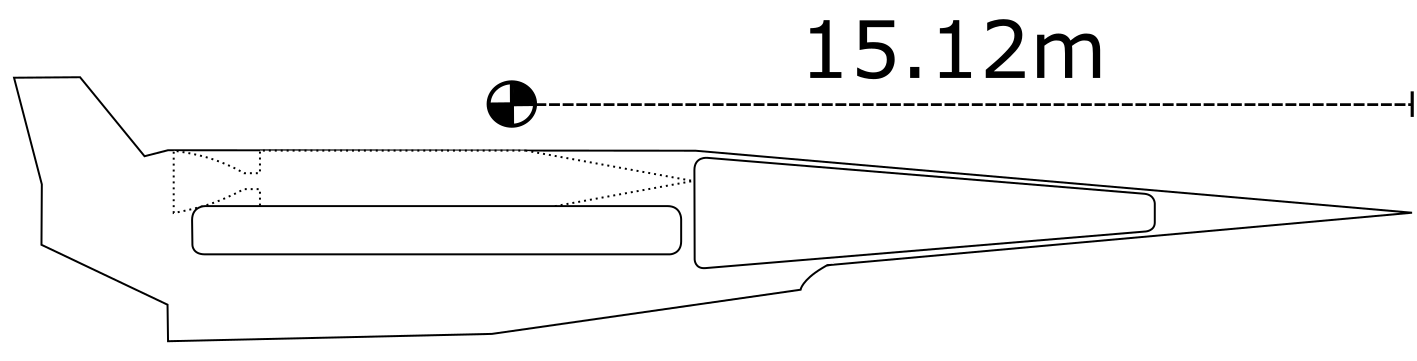
\includegraphics[width=0.9\linewidth]{figures/3_vehicle_design/CG5}
				\caption{Empty of fuel, after third stage release, engines off.}
				
			\end{subfigure}
			\caption{Centre of gravity positions throughout the flight of the scramjet accelerator. }%\textcolor{red}{XXX Changed}
			\label{fig:CentreOfGravity}
		\end{figure}
		
		
		\subsubsection{Calculation of Trimmed Flap Deflections}\label{sec:trim}
		
		
		\begin{figure}[ht]
			\centering
			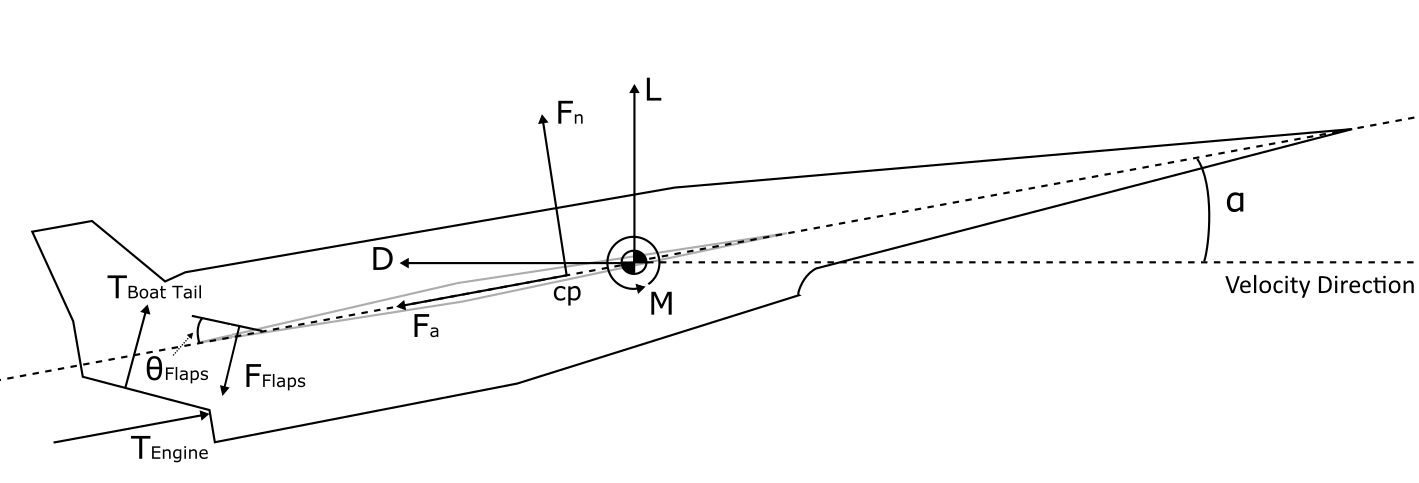
\includegraphics[width=0.7\linewidth]{figures/3_vehicle_design/SPARTANForces}
			\caption{The forces on the scramjet accelerator during flight.}
			\label{fig:SPARTANForces}
		\end{figure}
		
		The scramjet accelerator as designed by Preller\cite{Preller2017b} is trimmed using control surfaces on the wings, shown in figure \ref{fig:SPARTAN_FLAPS}. 
		The flaps of the scramjet accelerator are modelled at deflected states of -20$^\circ$, -10$^\circ$, 10$^\circ$, and 20$^\circ$. The scramjet accelerator is modelled in CREO with the flaps at each of these deflected states, and a surface mesh is created in Pointwise. 
		Cart3D is used to simulate each of these flap deflected states, and Clic is used to extract the aerodynamic coefficients, for Mach numbers between 0.2 and 10. These aerodynamic coefficients are tabulated, and interpolation splines fitted, so that the flight Mach number and the moment generated by the flaps are used to interpolate for the flap deflection, ie. $\theta_{Flaps} = f(M,M_{Flaps})$.
		\begin{figure}[ht]
			\centering
			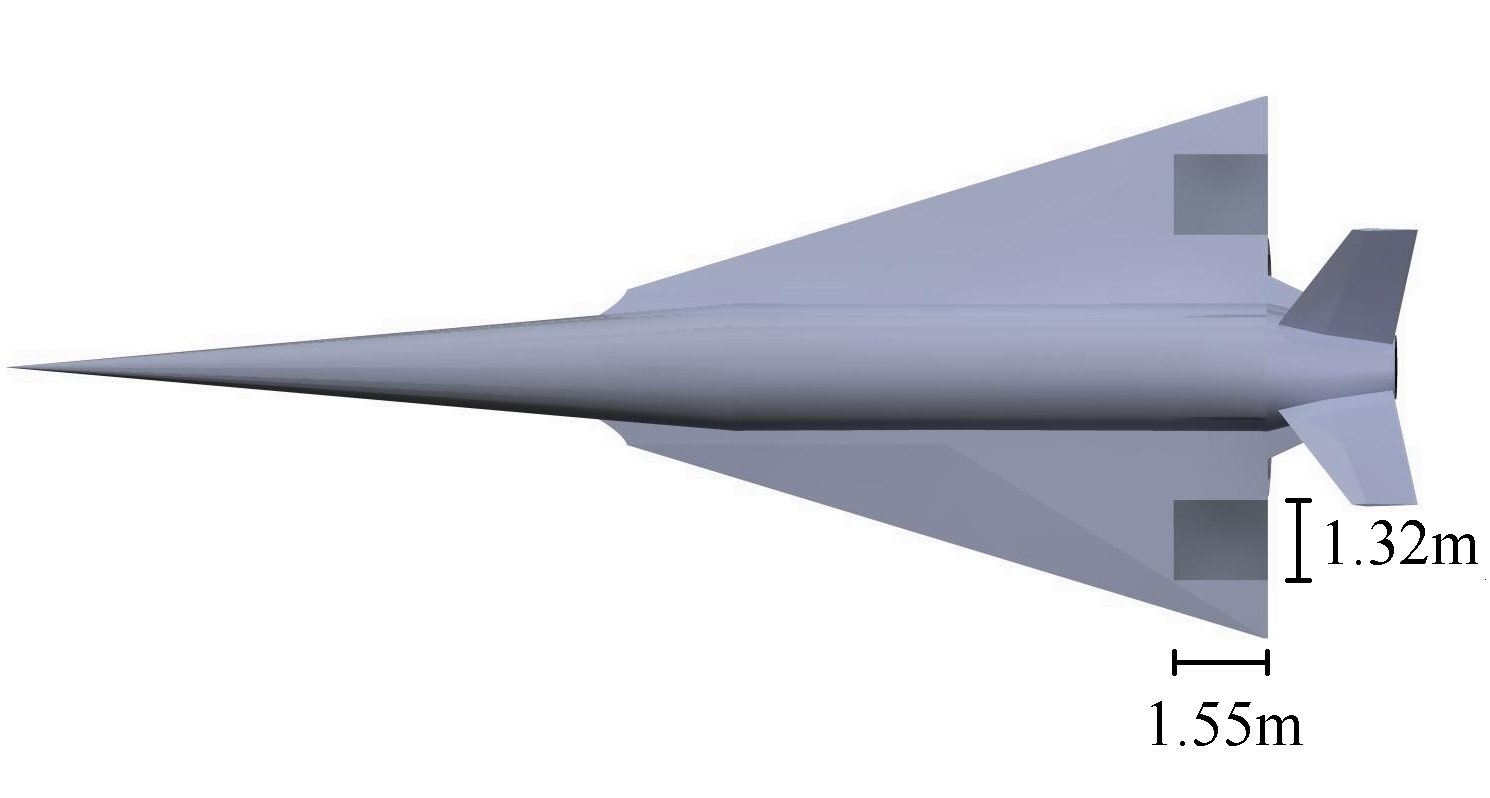
\includegraphics[width=0.6\linewidth]{figures/3_vehicle_design/SPARTAN_FLAPS}
			\caption{scramjet accelerator model showing control surfaces.}
			\label{fig:SPARTAN_FLAPS}
		\end{figure}
		Trim is determined by calculating the aerodynamic moment coefficient with zero flap deflection, then calculating the flap deflection necessary to balance the aerodynamic moments to zero. The moments generated by the untrimmed scramjet accelerator, as well as the thrust moments on the engines and boat tail when the C-REST engines are powered-on, are balanced by the moment generated by the flaps, so that:
		\begin{equation}
		M_{Flap} = -M_{Untrimmed}
		\end{equation}
		  
		
		 
		 
		

		
		
		
		\begin{figure}[ht]
			\begin{subfigure}{.5\textwidth}
				\centering
				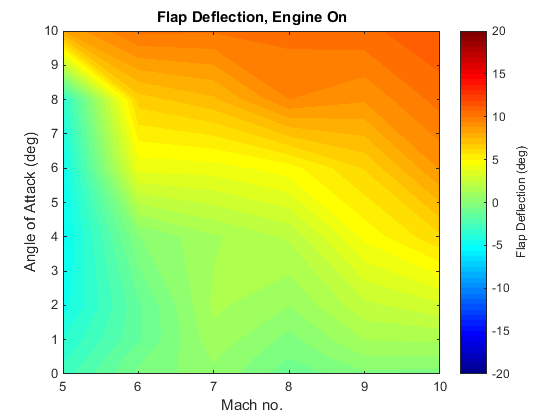
\includegraphics[width=0.99\linewidth]{figures/3_vehicle_design/FlapEngineCG1}
				\caption{Full of fuel, before third stage release.}
			\end{subfigure}
			\begin{subfigure}{.5\textwidth}
				\centering
				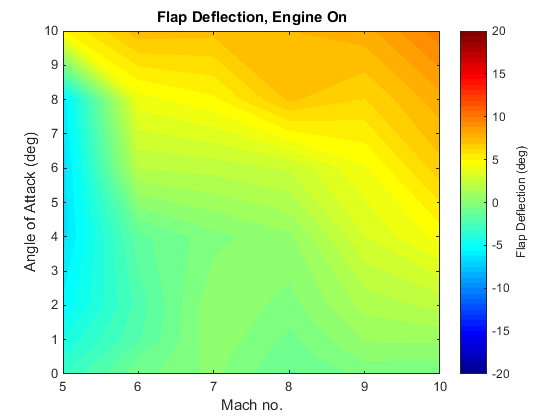
\includegraphics[width=0.99\linewidth]{figures/3_vehicle_design/FlapEngineCG2}
				\caption{After depletion of cylindrical fuel tanks, before third stage release.}
				
			\end{subfigure}
			\begin{subfigure}{.5\textwidth}
				\centering
				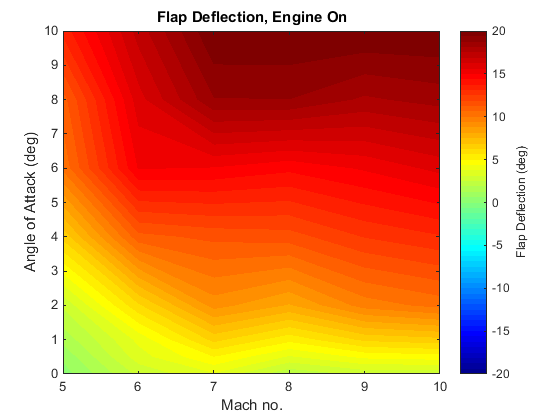
\includegraphics[width=0.99\linewidth]{figures/3_vehicle_design/FlapEngineCG3}
				\caption{Empty of fuel, before third stage release.}
				
			\end{subfigure}
			\begin{subfigure}{.5\textwidth}
				\centering
				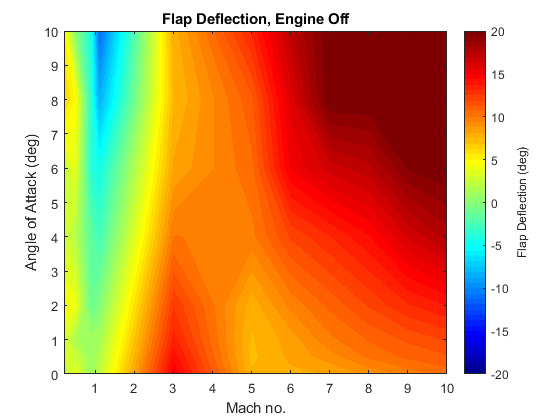
\includegraphics[width=0.99\linewidth]{figures/3_vehicle_design/FlapNoEngineCG4}
				\caption{Empty of fuel, after third stage release, engines off.}
				
			\end{subfigure}
			\caption{Flap deflection required for trim of the scramjet accelerator. Negative up.} % Updated 9/8/19
			\label{fig:FlapDeflection}
		\end{figure}
		
		The flap deflections necessary for trim are shown in Figure \ref{fig:FlapDeflection}, calculated for Mach numbers between 0.2 and 10, and at angles of attack from 0$^\circ$ to 10$^\circ$. Engine-on flap deflections are shown at centre of gravity locations corresponding to full-fuel, full conical tank, and empty conditions with the third stage included, and engine-off flap deflections are shown at the centre of gravity corresponding to a fuel-empty condition after third stage release. 
		The flap deflections are designated as negative up. Negative flap deflection necessary for trim indicates that the centre of pressure is aft of the centre of gravity, and that the vehicle has positive static margin.
		It can be observed that while the cylindrical fuel tanks are being used, the scramjet accelerator is generally stable at low angles of attack, and the static margin is close to 0, requiring only small flap deflections for trim. As the fuel in the conical tank is depleted, the centre of gravity moves aft, and the scramjet accelerator develops a negative static margin, requiring larger flap deflections to trim at high Mach numbers. These large flap deflections indicate that the scramjet accelerator may experience instability issues at the end of its acceleration, however, determining the controllability of the scramjet accelerator is outside the scope of this study. 
		
		  Once the flap deflections necessary to trim the scramjet accelerator are calculated, the additional lift and drag produced by the flaps are added to the aerodynamic database, ensuring that the scramjet accelerator is trimmed at every flight condition.
		  Trimmed aerodynamic databases are calculated for engine on and engine off conditions, as well as at all centre of gravity locations listed previously. 
		
		
		
		\subsubsection{Viscous Correction}
		
		\begin{figure}[ht]
			\begin{subfigure}{.5\textwidth}
				\centering
				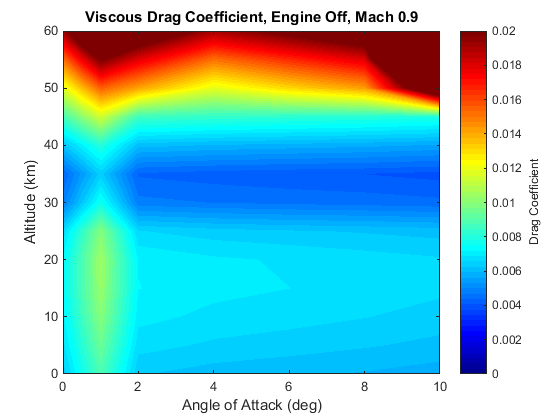
\includegraphics[width=0.99\linewidth]{figures/3_vehicle_design/ViscousCd1}
				\caption{Mach 0.9, engines off.}
			\end{subfigure}
			\begin{subfigure}{.5\textwidth}
				\centering
				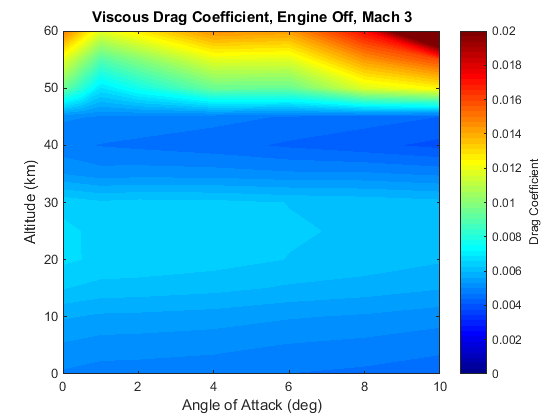
\includegraphics[width=0.99\linewidth]{figures/3_vehicle_design/ViscousCd2}
				\caption{Mach 3, engines off.}
				
			\end{subfigure}
			\begin{subfigure}{.5\textwidth}
				\centering
				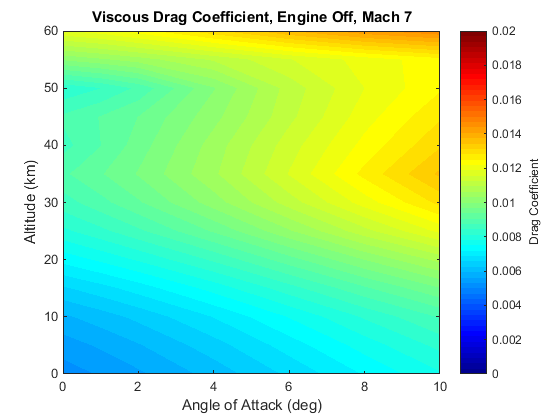
\includegraphics[width=0.99\linewidth]{figures/3_vehicle_design/ViscousCd3}
				\caption{Mach 7, engines off.}
				
			\end{subfigure}
			\begin{subfigure}{.5\textwidth}
				\centering
				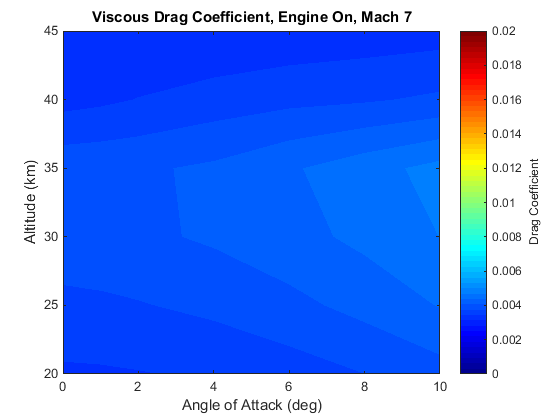
\includegraphics[width=0.99\linewidth]{figures/3_vehicle_design/ViscousCd4}
				\caption{Mach 7, engines on.}
				
			\end{subfigure}
			\caption{Viscous drag coefficient across various Mach numbers.}
			\label{fig:ViscousCd}
		\end{figure}
		As Cart3D is an inviscid solver, the aerodynamic database generated by Cart3D lacks the forces generated by skin friction drag. In order for the aerodynamic model to more closely approximate realistic dynamics, a correction for the viscous forces on the scramjet accelerator is calculated, using the viscous correction solver VC3D\cite{Ward2018}. VC3D utilises flat plate correlations for skin friction on each surface cell, employing a simplified running length based on the Euclidean distance to the respective stagnation feature. Further details of this solver can be found in Reference\cite{Ward2018}. This method has been shown to significantly improve upon the accuracy of the aerodynamic coefficients calculated by Cart3D for multiple test vehicles\cite{Ward2018}. The additional viscous force and moment components from flap deflections are calculated using mean skin friction coefficient for computational efficiency, due to the very small contribution of this to the flap forces. The viscous drag coefficients are generated for the scramjet accelerator at every Mach number and angle of attack which are simulated in Cart3D. Viscous databases are generated for both engine-on and engine-off cases, for altitudes of 20-45km and 0-60km respectively.  The viscous drag coefficients for selected flight conditions are shown in Figure \ref{fig:ViscousCd}.
		
		
		
		
		
		\subsection{Trimmed Aerodynamic Database of the Scramjet Accelerator with Engine-On}\label{sec:trimmedongineon}

		
		The engine-on aerodynamics of the scramjet accelerator are used during the simulation of the acceleration phase, when the C-REST engines are operational at all times, as well as during the fly-back phase, when the engines are operational for a short time to aid the scramjet accelerator in returning to its initial launch site.
		The external aerodynamics of the scramjet accelerator with the scramjet engines powered-on are calculated by removing the engine and boat tail from Cart3D simulations of the scramjet accelerator with engine flowpaths. Engine-on aerodynamic calculations are performed for Mach numbers 5,7,9 and 10. An example of a Cart3D solution of the nozzle exit and boat tail with the scramjet engines powered-on is shown in Figure \ref{fig:EngineOn}, and the aerodynamics of the scramjet accelerator with engines powered-on are shown in Figure \ref{fig:EngineOnAero}.
		
		
		\begin{figure}[ht]
			\centering
			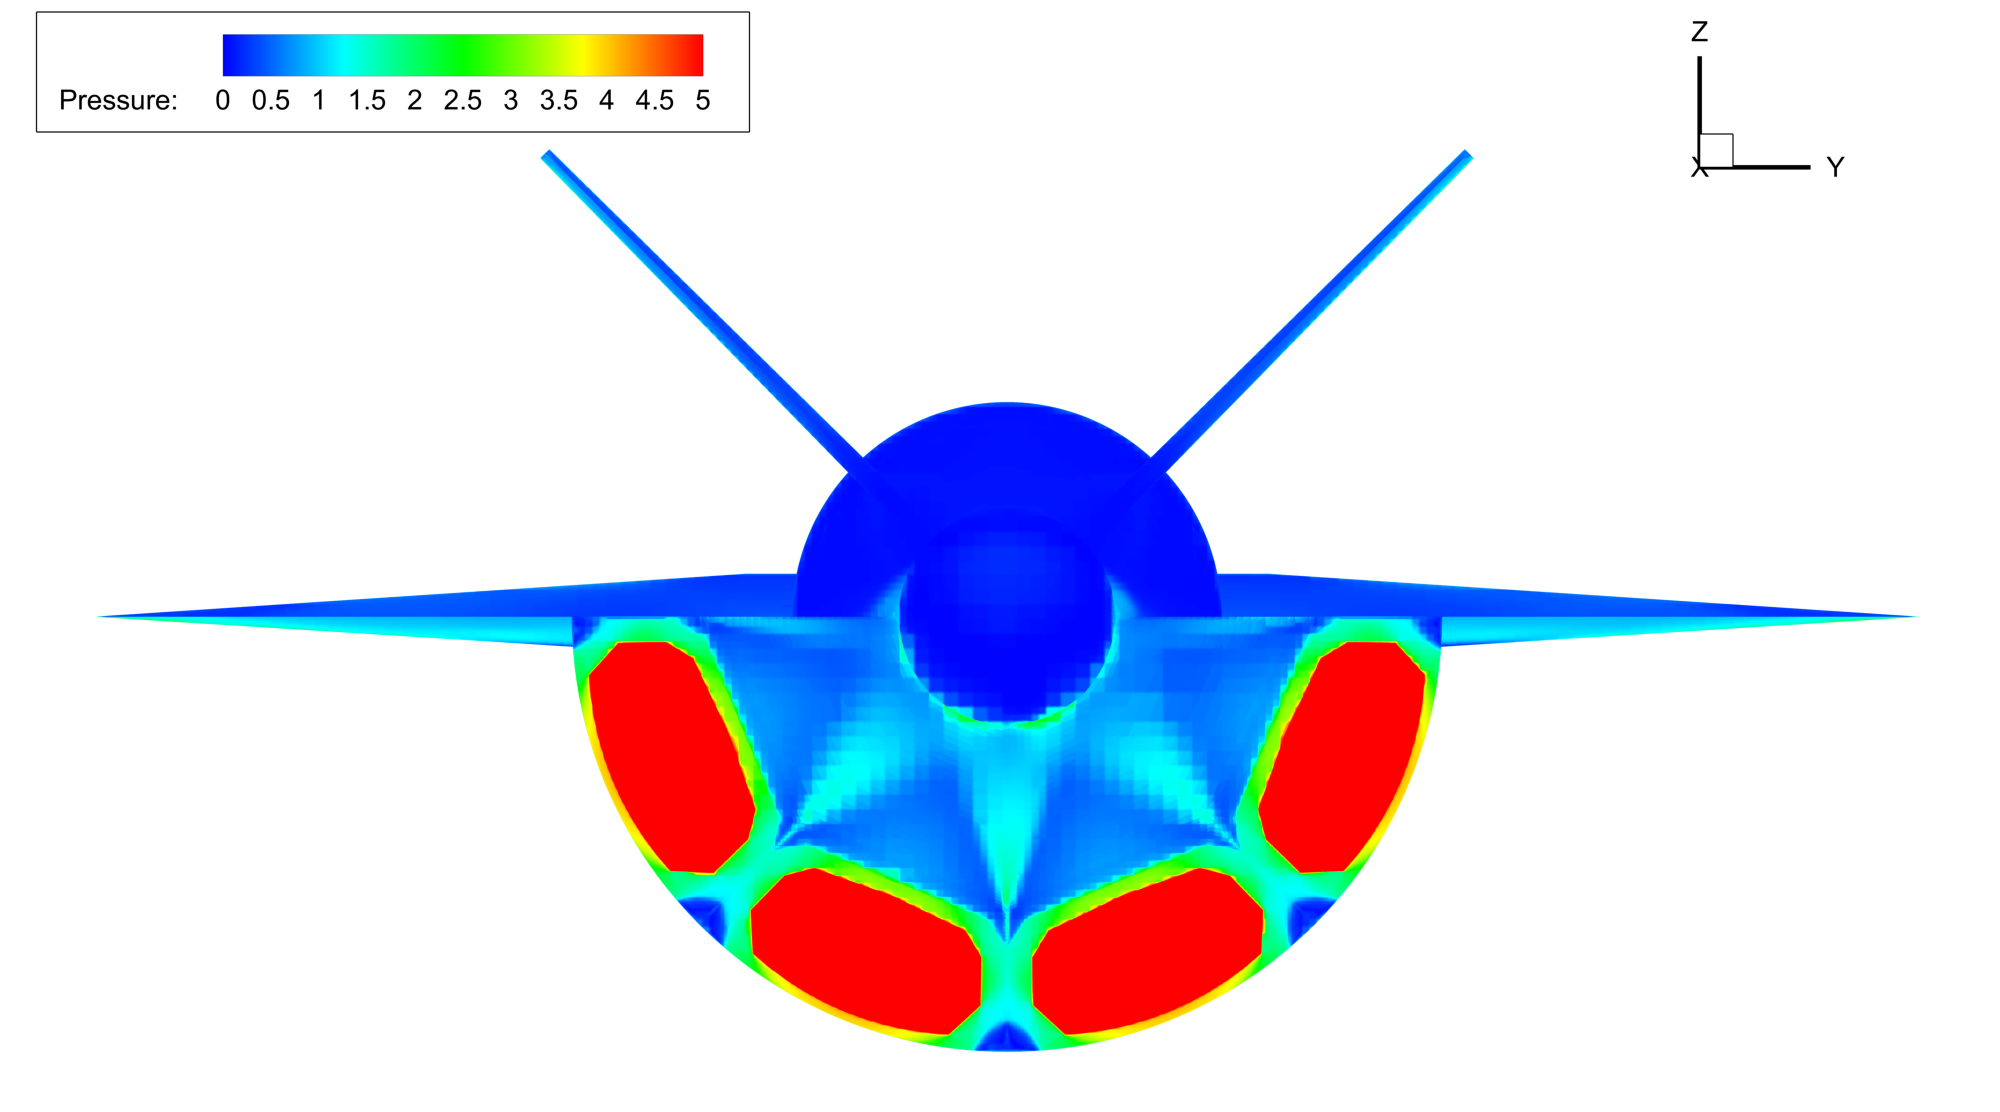
\includegraphics[width=0.9\linewidth]{figures/3_vehicle_design/EngineOn}
			\caption{Engine-on Cart3D simulation at Mach 6, 2$^\circ$ angle of attack, and 25km altitude.}
			\label{fig:EngineOn}
		\end{figure}
		
		
		\begin{figure}[ht]
			\begin{subfigure}{.5\textwidth}
				\centering
				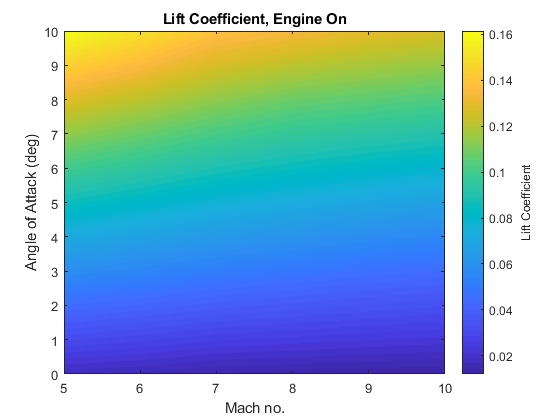
\includegraphics[width=0.99\linewidth]{figures/3_vehicle_design/Cl-EngineOn}
				\caption{Coefficient of lift.}
				\label{fig:Cl-EngineOn}
			\end{subfigure}
			\begin{subfigure}{.5\textwidth}
				\centering
				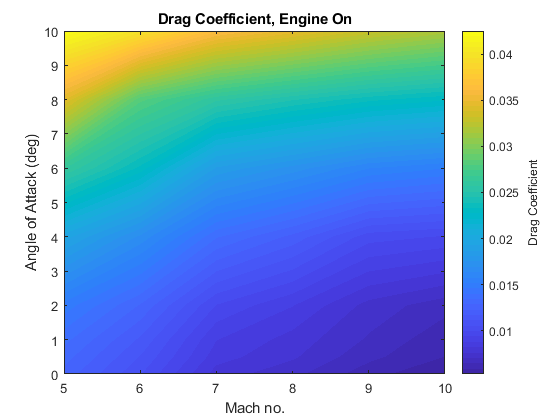
\includegraphics[width=0.99\linewidth]{figures/3_vehicle_design/Cd-EngineOn}
				\caption{Coefficient of drag.}
				\label{fig:Cd-EngineOn}
			\end{subfigure}
			\begin{subfigure}{.5\textwidth}
				\centering
				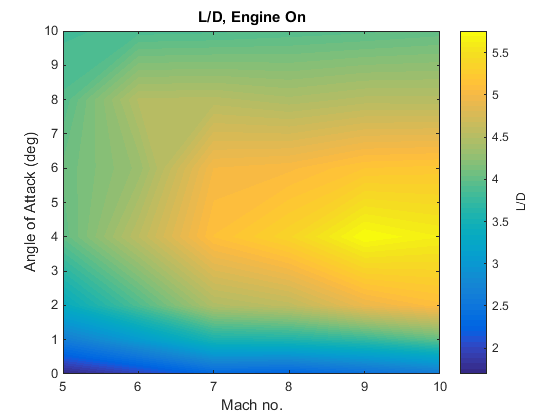
\includegraphics[width=0.99\linewidth]{figures/3_vehicle_design/LD-EngineOn}
				\caption{L/D.}
				\label{fig:LD-EngineOn}
			\end{subfigure}
			\caption{The aerodynamic coefficients of the scramjet accelerator with the C-REST engines powered-on at 30km altitude. Coefficients correspond to a reference area of 62.77m$^2$ and a centre of gravity of \textcolor{red}{15.24m} (full of fuel, with third stage). }% updated 9/8/29
			\label{fig:EngineOnAero}
		\end{figure}
		
		

\subsection{Trimmed Aerodynamic Database of the Scramjet Accelerator with Engine-Off}\label{sec:trimmedongineoff}

\begin{figure}[ht]
\begin{subfigure}{.9\textwidth}
	\centering
	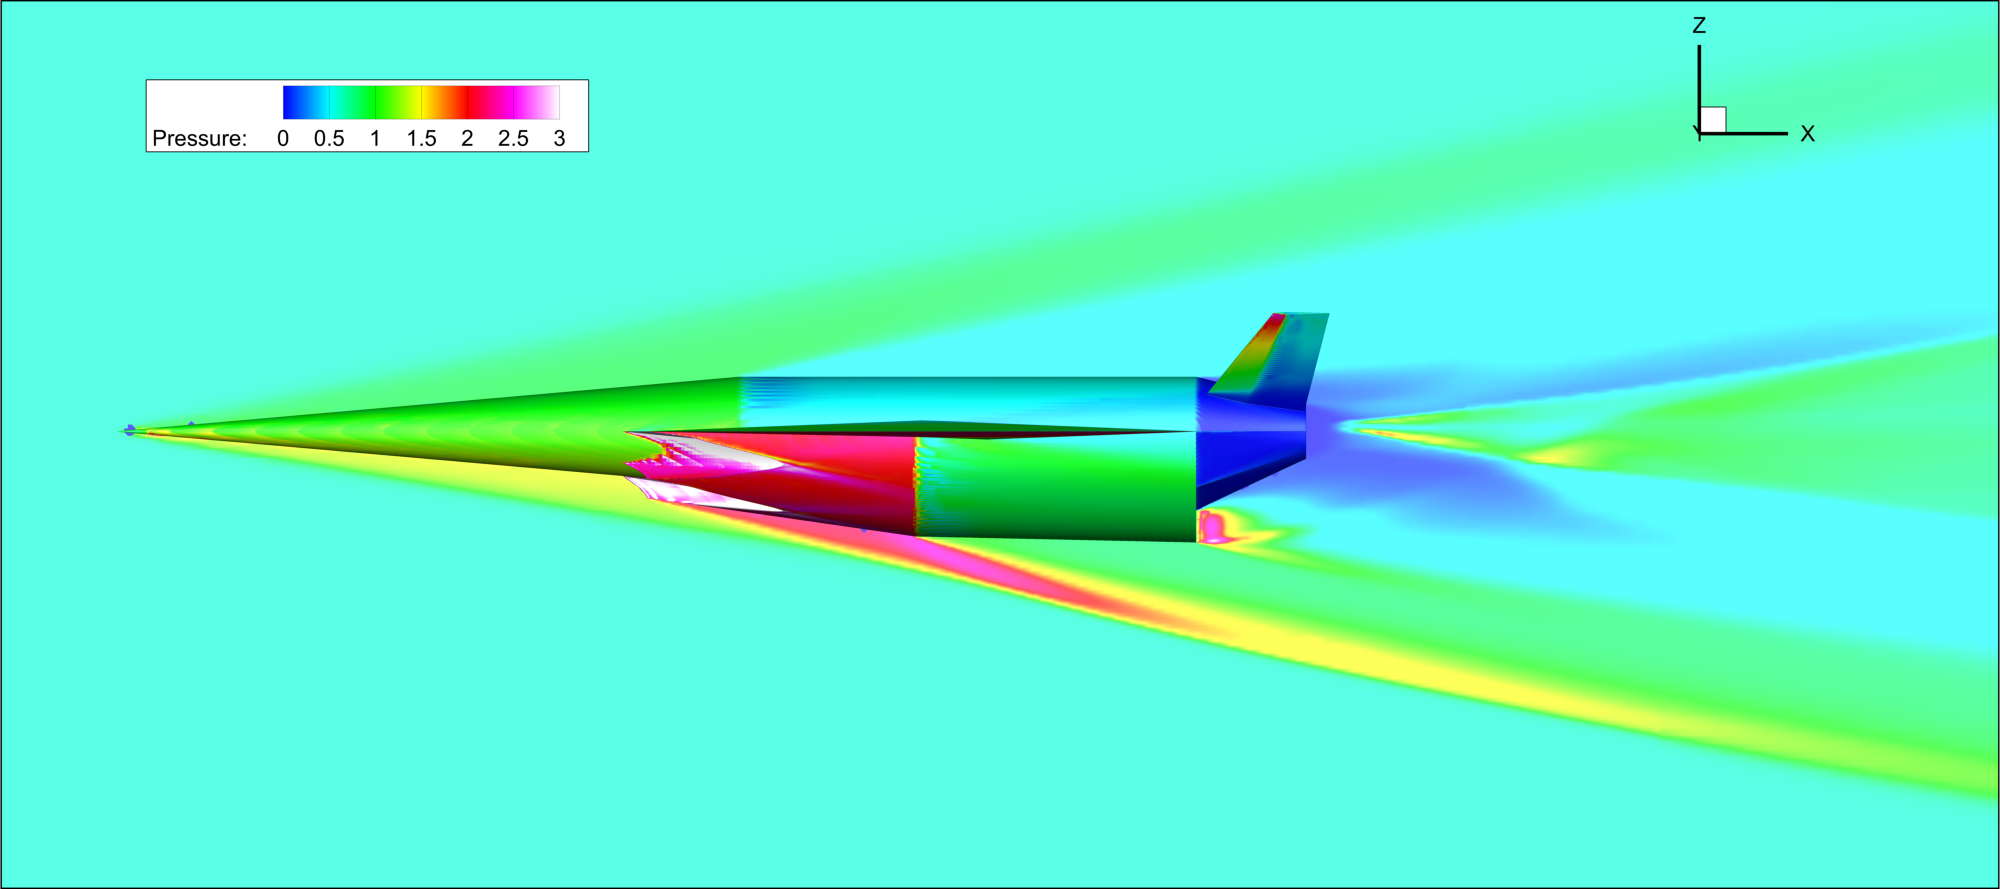
\includegraphics[width=0.9\linewidth]{figures/3_vehicle_design/CartSide}
	\caption{Side view.}
	\label{fig:CartSide}
\end{subfigure}

\begin{subfigure}{.9\textwidth}
	\centering
	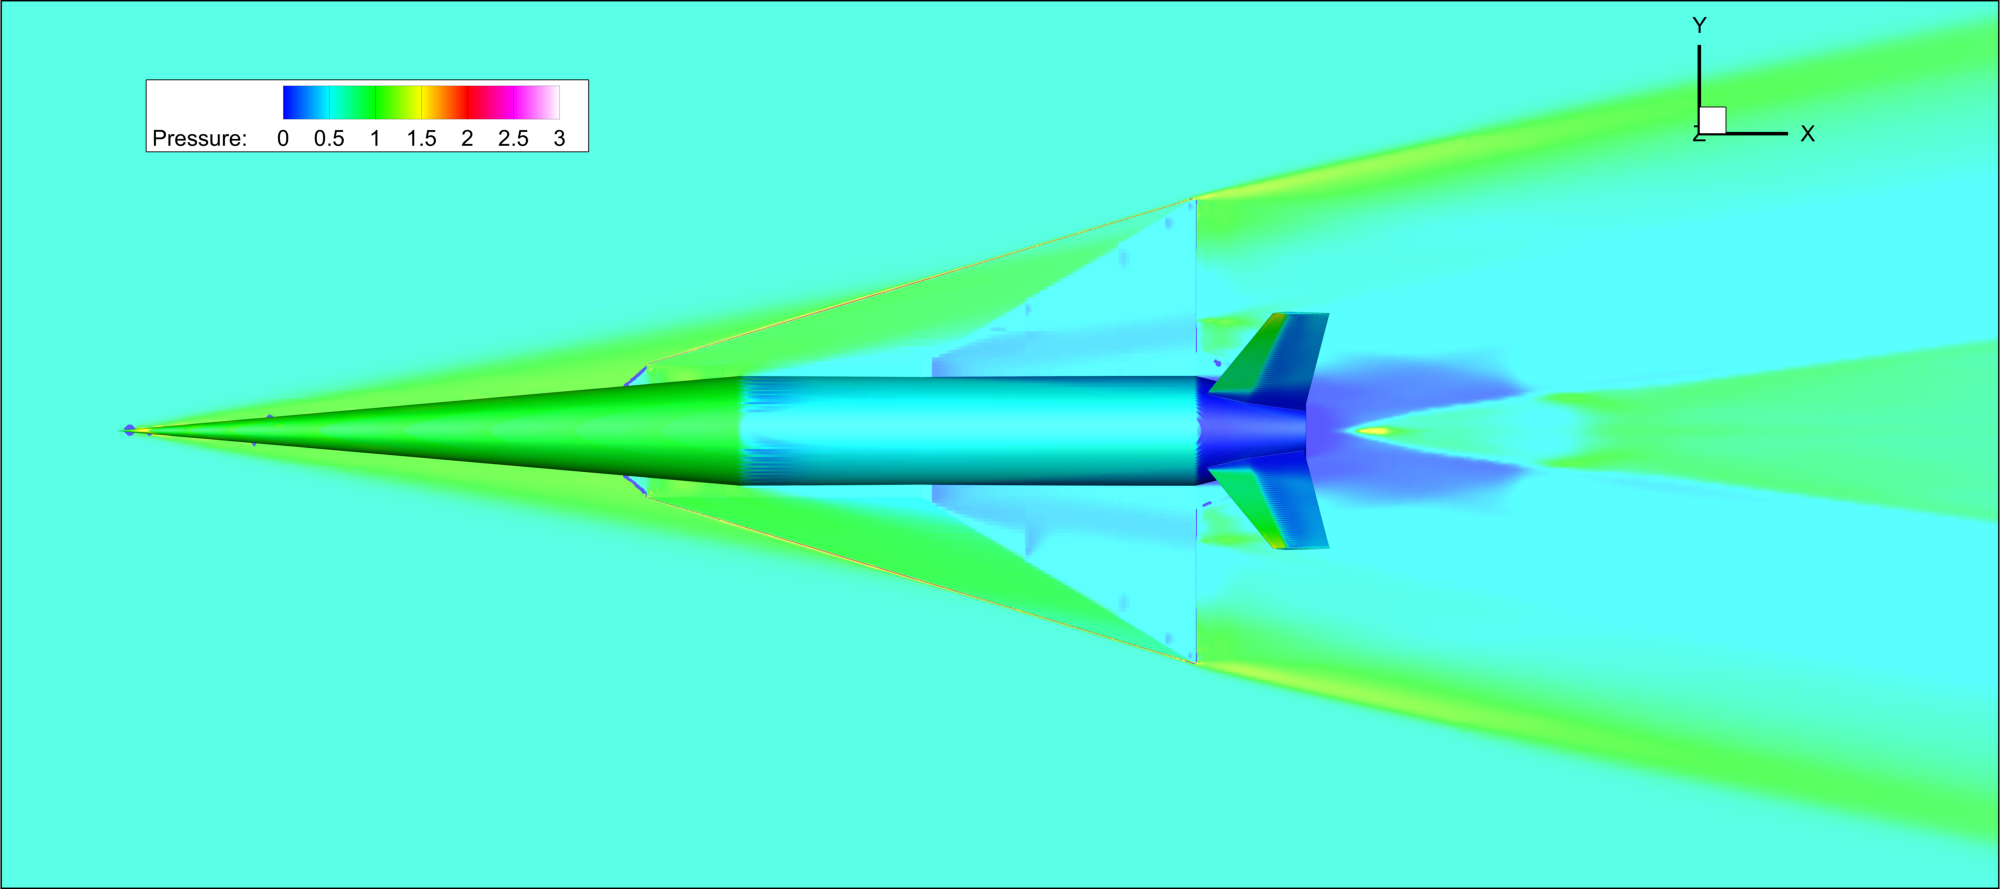
\includegraphics[width=0.9\linewidth]{figures/3_vehicle_design/CartTop}
	\caption{Top view.}
	\label{fig:CartTop}
\end{subfigure}
\caption{Cart3D flow result for the scramjet accelerator, at Mach 6, 2$^\circ$ angle of attack.}
\label{fig:CartSPART}
\end{figure}

\begin{figure}[ht]
	\begin{subfigure}{.5\textwidth}
		\centering
		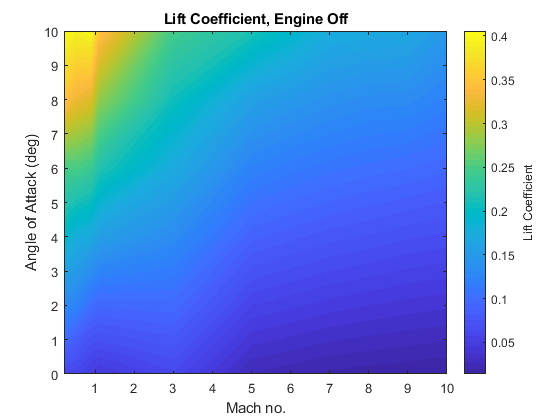
\includegraphics[width=0.99\linewidth]{figures/3_vehicle_design/Cl}
		\caption{Coefficients of lift of the scramjet accelerator, calculated using Cart3D.}
		\label{fig:Cl}
	\end{subfigure}
	\begin{subfigure}{.5\textwidth}
		\centering
		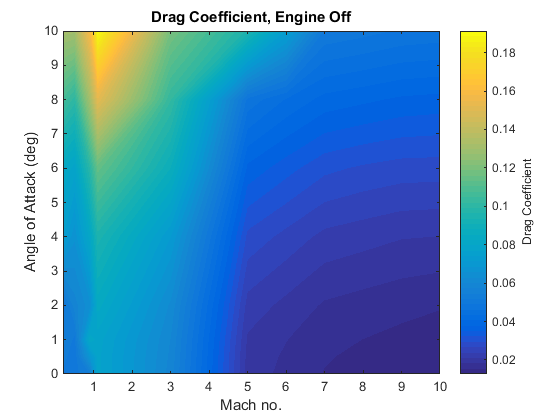
\includegraphics[width=0.99\linewidth]{figures/3_vehicle_design/Cd}
		\caption{Coefficients of drag of the scramjet accelerator, calculated using Cart3D.}
		\label{fig:Cd}
	\end{subfigure}
	\begin{subfigure}{.5\textwidth}
		\centering
		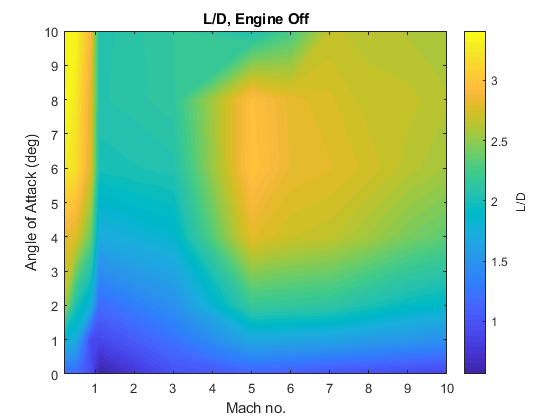
\includegraphics[width=0.99\linewidth]{figures/3_vehicle_design/LD}
		\caption{L/D of the scramjet accelerator.}
		\label{fig:LD}
	\end{subfigure}
	\caption{Aerodynamic Characteristics of the scramjet accelerator with C-REST engine powered-off at an altitude of 30km. Coefficients correspond to a reference area of 62.77m$^2$ and a centre of gravity of 15.16m (no third stage, no fuel).} % updated 9/8/19
	\label{fig:aero1}
\end{figure}

During the majority of the return flight, the scramjet engines are not operational, and the scramjet accelerator is gliding without power. The return phase takes the scramjet accelerator from third stage separation, at approximately Mach 9, to landing approach at low subsonic speeds. 
 While the engines are not powered-on air flows through the flowpath without fuel injection, generating a large amount of drag. 
The aerodynamics of the scramjet accelerator are calculated using Cart3D for Mach numbers from 0.2 to 10, and angle of attack values from 0$^\circ$ to 10$^\circ$ to cover the range of flight conditions experienced during the fly-back of the scramjet accelerator.  An example Cart3D solution is shown for a Mach 7 engine off condition in Figure  \ref{fig:CartSPART}. \textcolor{red}{A strong bow shock can be observed, as well as a large shock from the underside of the vehicle, generated by the engine cowl. It can be observed that the aerodynamic pressure is extremely high on the angled portion of the engine cowl, due to its high incident angle to the incoming flow. Significantly high pressure is also experienced by the nose cone and cowl underside, as well as on a section of the tail, where a small shock generated by the wings is incident on the tail.}
Figure \ref{fig:aero1} shows the engine off aerodynamic characteristics of the scramjet accelerator vehicle over the range of Mach numbers and angle of attack values analysed.
These results show a distinct maximum region in the L/D of the scramjet accelerator at high Mach numbers, within the hypersonic regime. Below Mach 5, the L/D of the scramjet accelerator decreases sharply. This is caused by the scramjet engines unstarting, generating significant drag. The unstarted scramjet engines are shown in Figure \ref{fig:Unstart}\textcolor{red}{, where shocks within the inlet of the engine are evident, causing high pressures}. Below Mach 3,  the L/D shows a trend of general increase, except at very low angle of attack, as the effects of the unstarted engine lessen. Below Mach 1 the L/D of the scramjet accelerator increases significantly, in part due to not having the significant drag induced from the engines unstarting, as observed in the supersonic regime.  

\begin{figure}[ht]
	\centering
	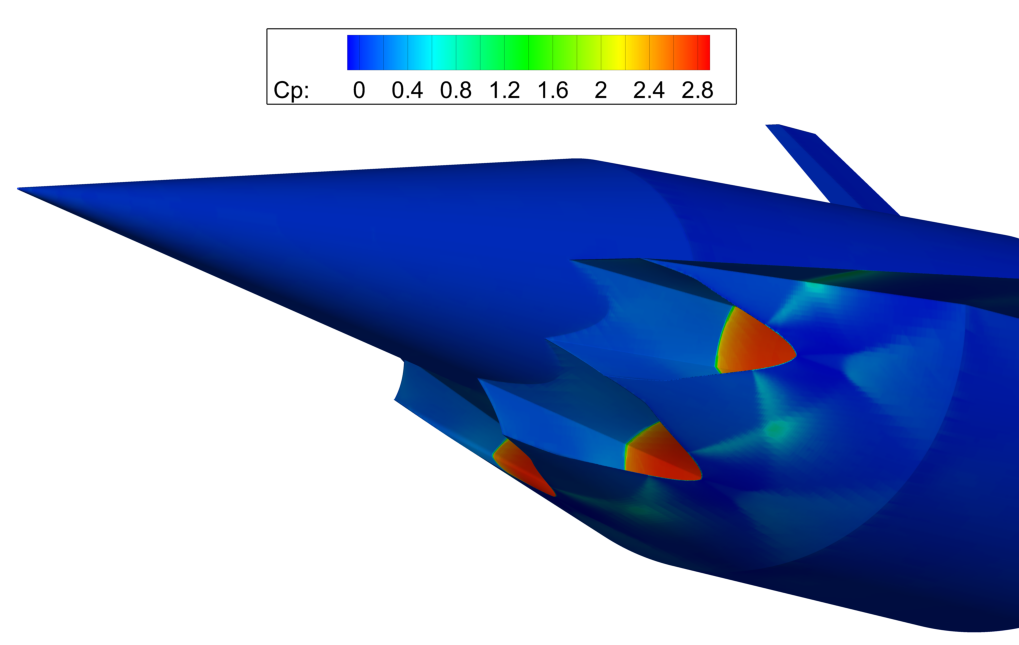
\includegraphics[width=0.7\linewidth]{figures/3_vehicle_design/Unstart}
	\caption{Unstarted scramjet engines at mach 3, 2$^\circ$ angle of attack.}
	\label{fig:Unstart}
\end{figure}


\section{The First Stage Rocket}\label{sec:firststage}



The first stage rocket is required to deliver the second stage to near horizontal flight at Mach 5.1 flight conditions,
after which it is discarded. 
\textcolor{red}{The representative first stage rocket in this study has been  modelled as a Falcon-1e first stage scaled down
lengthwise to 9.5m and to a mass of 1800kg, keeping the original diameter of 1.67m\cite{Vehicle2008}. This scaling was based off a first principles design of the first stage mass and performance necessary to achieve the minimum operating conditions of the scramjet accelerator, performed by Preller \& Smart\cite{Preller2017b}, with some tuning due to the higher fidelity aerodynamics used in this study.}
The Falcon-1e has been chosen due to its appropriate scale, and the proven flightworthiness of the Falcon-1. 
 The first stage is attached to the rear of the scramjet
second stage and is powered by a single LOX-kerosene Merlin 1-C engine. A connecting cowl has been modelled between the first stage rocket and the scramjet accelerator to improve the aerodynamic profile.  The first stage has a structural mass of
\textcolor{red}{820.5}kg, determined by scaling of the structural mass of the Falcon-1e. The engine mass of the Merlin 1-C is kept constant during scaling at 630kg\cite{Wade2017}. The mass of the
fuel in the first stage is scaled as part of the optimisation routine, as the dynamics of the vehicle, and its ability to reach a
given separation point, are very closely coupled to the available fuel mass.

\begin{table}[!h]
	\centering
	\begin{tabular}{|c|c|}
		\hline  $I_{SP_{SL}}$ & 275s \\ 
		\hline  $I_{SP_{vac}}$ & 304s\\ 
		\hline  $T_{SL}$ & 555.9kN \\ 
		\hline  $A_{e}$ & $0.552m^2$ \\ 
		\hline 
	\end{tabular} 
	\caption{First Stage Engine Properties\cite{Wade2017}.}
	\label{tab:1stStageEngine}
\end{table}
The thrust and specific impulse of the Merlin 1-C are determined by interpolation between the sea level and vacuum specific impulse of the Merlin 1-C, shown in Table \ref{tab:1stStageEngine}, with ambient pressure. Thrust scaling is determined by linear pressure scaling using nozzle exit area, $T = T_{SL} + (p_e - p_{SL})A_e$. 
 \textcolor{red}{The Merlin 1-C is throttlable between 70\% and 100\%\cite{Norris2011}}.




  \subsection{The Aerodynamics of the First Stage Rocket and Scramjet Accelerator}\label{sec:firststageaero}
  
  
  
  
   \begin{figure}[ht]
   	\centering
   	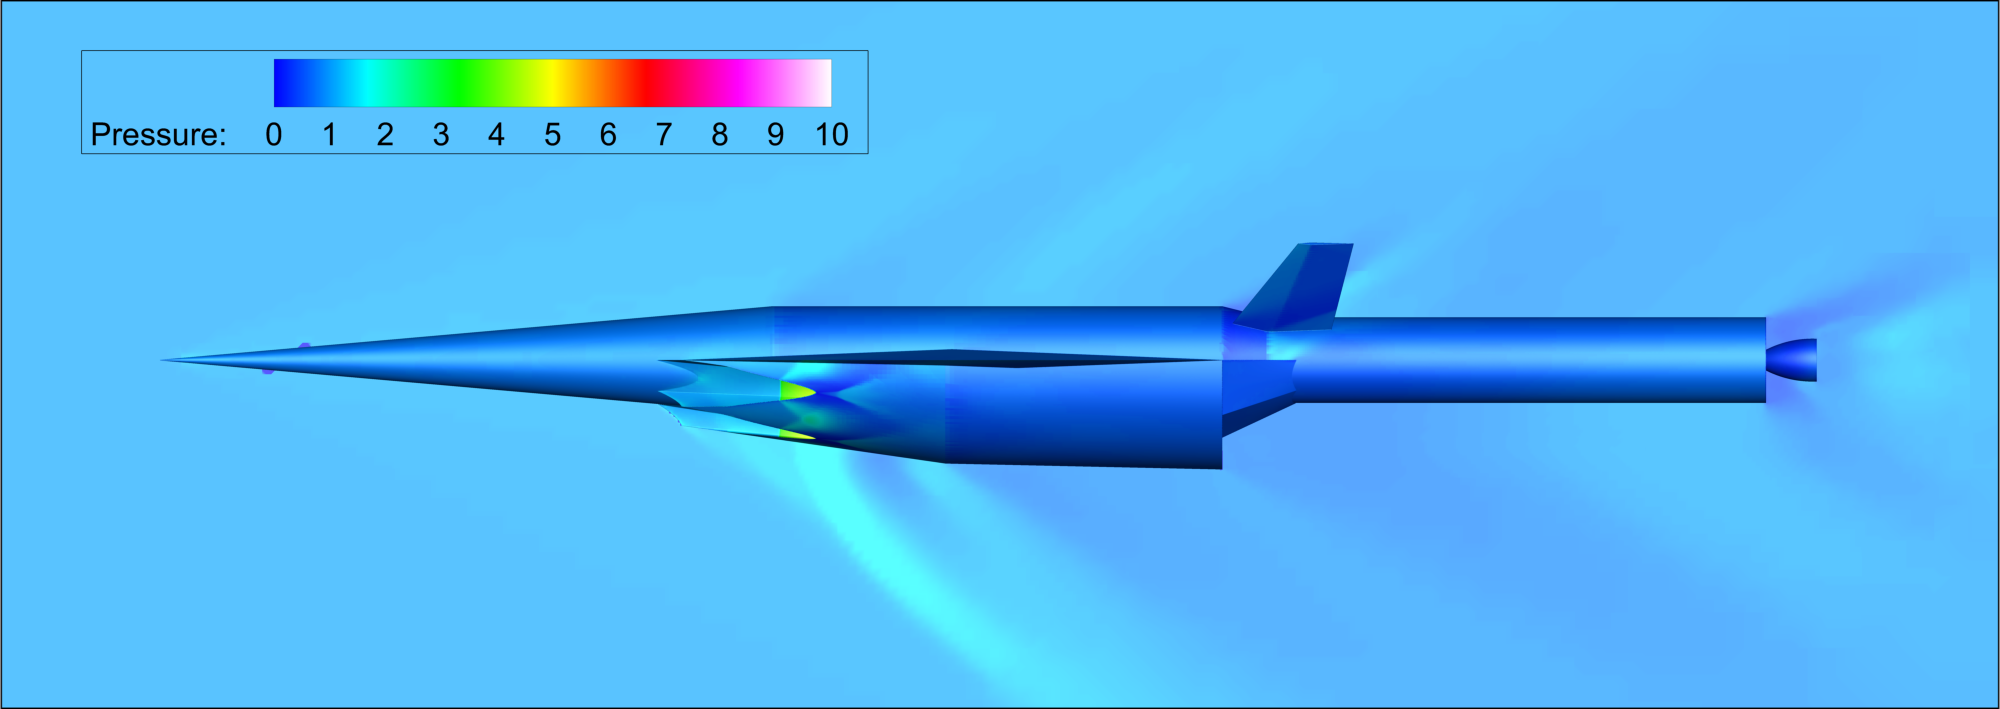
\includegraphics[width=0.8\linewidth]{figures/3_vehicle_design/CARTcontour}
   	\caption{Cart3D result for the scramjet accelerator and first stage vehicles at Mach 2, -1$^\circ$ angle of attack.}
   	\label{fig:CARTcontour}
   \end{figure}
   
    
    \begin{figure}[ht]
    	\begin{subfigure}{.5\textwidth}
    		\centering
    		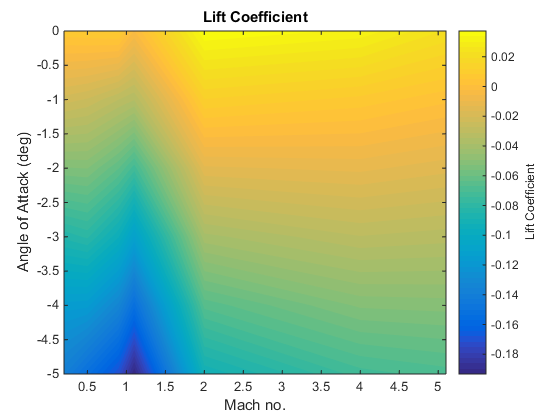
\includegraphics[width=0.99\linewidth]{figures/3_vehicle_design/FirstStageCl}
    		\caption{Coefficient of lift.}
    		\label{fig:Cl-FirstStage}
    	\end{subfigure}
    	\begin{subfigure}{.5\textwidth}
    		\centering
    		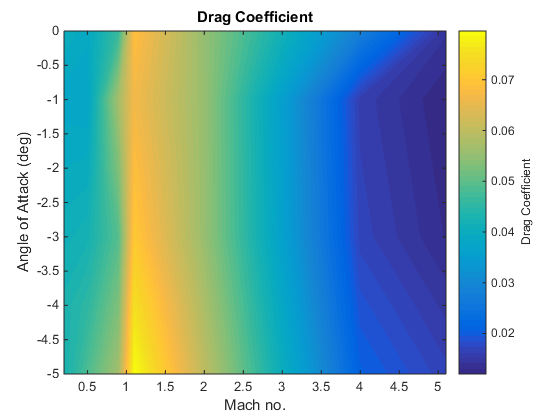
\includegraphics[width=0.99\linewidth]{figures/3_vehicle_design/FirstStageCd}
    		\caption{Coefficient of drag.}
    		\label{fig:Cd-FirstStage}
    	\end{subfigure}
    	\begin{subfigure}{.5\textwidth}
    		\centering
    		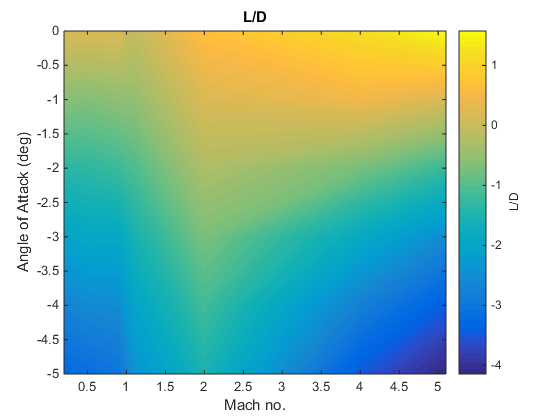
\includegraphics[width=0.99\linewidth]{figures/3_vehicle_design/FirstStageLD}
    		\caption{L/D.}
    		\label{fig:LD-EFirstStage}
    	\end{subfigure}
    	\caption{The aerodynamic characteristics of the SPARTAN stack.  Coefficients correspond to a reference area of 62.77m$^2$.}
    	\label{fig:FirstStageAero}
    \end{figure}
  The aerodynamics of the launch system during first stage flight are calculated in a similar manner to those of the scramjet accelerator without the first stage rocket, as detailed in Section \ref{sec:aero}. 
  The aerodynamics of the scramjet accelerator and first stage rocket are calculated using Cart3D and corrected for viscous effects. The first stage aerodynamics are modelled between angles of attack of 0$^\circ$ to -5$^\circ$, as the first stage will be flying at negative angle of attack to induce faster pitch-over. Mach numbers from 0.2 to 5.1 (second stage separation velocity) are simulated. Figure \ref{fig:CARTcontour} shows an example Cart3D simulation case, at Mach 2, -1$^\circ$ angle of attack. The coefficient of lift, drag and aerodynamic moment are tabulated for each simulation. Figure \ref{fig:FirstStageAero} shows the lift and drag coefficients of the first stage, as well as the lift-over-drag, across the simulated Mach Numbers and angles of attack. Above -1$^\circ$ angle of attack, the L/D of the first stage is generally greater than 0, meaning that lift is being gained in the positive vertical direction, and that the angle of attack must be lower than 1$^\circ$ to assist pitching.
  At Mach numbers over Mach 2, the absolute magnitude of the L/D generally increases as the Mach number increases. This is caused by the decreased effects of the engines unstarting, in turn reducing the drag of the engines at higher Mach numbers, as observed in the aerodynamics of the scramjet accelerator in Section \ref{sec:SPARTAN}. 
   Note that absolute magnitude is the metric used for `good' L/D, as the angles of attack are negative. 
  
  The First stage is trimmed using thrust vectoring of the Merlin 1-C engine during flight. The centre of gravity of the launch system varies from 23.8m to 16.8m along the vehicle, as the fuel of the first stage is depleted. The thrust vector angle of the engine is adjusted so that the moment caused by the rocket engine is equal and opposite to the moment caused by the aerodynamics of the vehicle, as illustrated in Figure \ref{fig:FirstStageThrustVec}, ie. $M_T = -M_{Fn}$.
  This thrust vectoring is calculated as the trajectory is simulated, at every flight condition. 
 

\begin{figure}
\centering
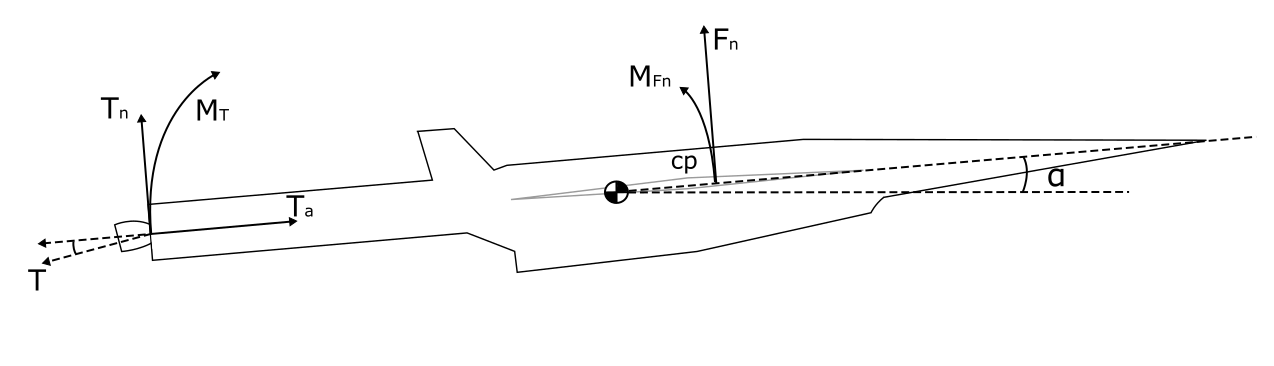
\includegraphics[width=0.9\linewidth]{figures/3_vehicle_design/FirstStageThrustVec}
\caption{Thrust vectoring moment balancing of the first stage.}
\label{fig:FirstStageThrustVec}
\end{figure}
  
  
  



	

	\textcolor{red}{\section{The Third Stage Rocket}\label{sec:ThirdStageBaseline}}

	\begin{figure}
\centering
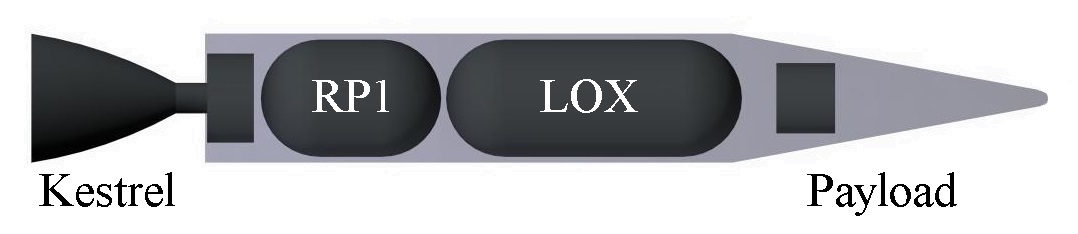
\includegraphics[width=0.7\linewidth]{figures/3_vehicle_design/3rdStage}
\caption{The third stage rocket, showing major internal features. }
\label{fig:3rdStage}
\end{figure}

The third stage rocket is an expendable portion of the launch system, tasked with delivering the payload to its final orbital position. 
  The third stage is released from the scramjet accelerator at a flight speed of approximately Mach 9, after which it must fly within the atmosphere for a time, performing a significant altitude raising manoeuvre to achieve orbital flight\cite{Preller2017b}. 
  In previous studies, the third stage of the SPARTAN was designed around a pump-fed RL-10-3A engine\cite{Preller2017b}, and was designed to fit into a cavity on the back of the fuselage of the vehicle\cite{Preller2017b}. For the representative launch vehicle in this work a new third stage is designed, to reduce cost, and to integrate within the fuselage of the scramjet accelerator. 
   
  The third stage rocket in this study is designed around a modified version of the SpaceX Kestrel engine. The Kestrel is a pressure-fed engine, which was designed for launching small satellites to orbit as part of the now retired Falcon-1. The Kestrel is chosen primarily for its low cost, to ensure that the representative launch system in this study closely approximates a cost-effective future launch system.  
  The third stage rocket in this study has a total length of \textcolor{red}{8.66}m, and is sized so that it is able to fit within the main cylindrical fuselage section of the scramjet accelerator's geometry.  This is done to reduce the heat loads present on the third stage during the second stage acceleration, as well as to improve the aerodynamics of the scramjet accelerator during ascent and fly-back. While the release mechanism of the third stage is not considered in this study, it is assumed that the release process will be simplified if the release mechanism is constrained to the cylindrical fuselage of the scramjet accelerator, rather than involving geometric variation of the nose cone of the scramjet accelerator, which receives a large amount of aerodynamic force as illustrated in Figure \ref{fig:CartTop}.
  
 The third stage internals have been designed to weigh a total of 3300kg. This has been chosen as a nominal design weight, to satisfy the fuel necessary to achieve orbit with an acceptable payload, while also allowing for ample payload volume. The internal layout of the third stage rocket is shown in Figure \ref{fig:3rdStage}, and a mass breakdown is given in Table \ref{tab:MassBreakdown3}. The third stage has a structural mass fraction of 0.079, to match the Falcon 1 second stage without the Kestrel engine or fairing included\cite{Vehicle2008}. This gives a total structural mass of 236.3kg, without heat shield or engine. 
 

 
	\begin{table}[h]
		\centering
		\begin{tabular}{|c|c|c|c|c|c|c|}
			\hline  \textbf{Part} & Total & Structural & Heat Shield & Engine & Fuel & Payload (est) \\ 
			\hline \textbf{Mass} (kg) & 3300.0  & 236.3  & 124.6  & 78.0  & 2761.1 & 100.0\\ 
			\hline 
		\end{tabular} 
		\caption{Mass breakdown of the third stage rocket.} % updated 12/8/19
		\label{tab:MassBreakdown3}
	\end{table}
 
 
 
 
 \subsection{Geometry}\label{sec:3int}

The third stage has a total length of 9m, to fit within the main body fuselage of the scramjet accelerator.
 The third stage nose length is set at 3m, for a similar nose geometry to the third stage designed for previous analysis of the scramjet accelerator\cite{Preller2017b}. This nose geometry is chosen so that the heat shield in this study may be appropriately modelled after the heat shield designed for the Rl-10-3A-powered third stage\cite{Preller2017b}.
 The third stage centrebody length has been set to 4.5m, giving a total length of 9m, with a 1.9m long Kestrel engine\cite{Vehicle2008}. The diameter of the third stage has been set to 1.1m including heat shield, to match the diameter of the Kestrel engine, and to be close to half the diameter of the scramjet accelerator, a scale used to fix the third stage width of the Rl-10-3A powered third stage\cite{Preller2017b}.  






	


\subsection{Fuel Tank Sizing}


The internal design of the third stage is allowed to be slightly variable as the trajectory is optimised. The third stage mass is fixed at 3300kg, and the calculated payload-to-orbit varies by exchanging leftover fuel mass for effective payload mass. The Kestrel engine utilises LOX/RP-1 propellants, with an oxidiser-to-fuel mixture ratio 2.56\cite{RPE} and a density of 813kg/m$^3$\cite{Magee}. 
To calculate the dynamics of the third stage, the fuel tanks have been approximately sized, assuming \textcolor{red}{100kg} of payload-to-orbit. Realistically the exchange between fuel and payload mass would cause the fuel tanks to be resized slightly, however, for the purposes of this study the fuel tanks are assumed to be of constant size for simplicity. Currently this is a reasonable assumption as the internals of the rocket are very simplified. With an assumed payload mass of \textcolor{red}{100kg}, the third stage carries a total propellant mass of \textcolor{red}{2761.1kg}. Table \ref{tab:Fuel} breaks shows the component break-down of the LOX oxidiser and RP1 for this fuel weight. The total mass and volumes of these fuels will change slightly as the trajectory of the launch system is optimised, and fuel is traded for payload mass. However, the ratio between the fuel and oxidiser will stay constant. 

	

\begin{table}[h]
	\centering
	\begin{tabular}{|c|c|c|}
		\hline  & \textbf{LOX} & \textbf{RP1} \\ 
		\hline Ratio & 2.56\cite{RPE} & 1 \\ 
		\hline Density & 1141kg/m3 & 813kg/m3\cite{Magee}\\ 
		\hline Volume & \textcolor{red}{1.740m$^3$} & \textcolor{red}{0.954m$^3$} \\ 
		\hline Mass & \textcolor{red}{1985.5} kg & \textcolor{red}{775.6} kg \\ 
		\hline 
	\end{tabular} 
	\caption{Third stage fuel distribution.} % updated 21/8/19
	\label{tab:Fuel}
\end{table}



\subsection{Heat Shield Sizing}
XXX change cork density/thickness

The third stage rocket is separated from the scramjet accelerator at a high dynamic pressure, after which it spends some time accelerating in-atmosphere before reaching exoatmospheric conditions. The time spent within a high dynamic pressure environment creates a large amount of heat loading, which must be mitigated by heat shielding. The heat shielding must be capable of withstanding the extremely high heat and structural loading necessary to protect the third stage rocket internals and payload, as well as being lightweight, as the payload-to-orbit is extremely sensitive to the mass of the third stage, and cost effective, as increasing the cost of the third stage directly increases launch cost due to it being expendable. 


The heat shield used to protect the third stage is constructed from a tungsten nose tip, a reinforced carbon-carbon nose cone, and a phenolic cork cylinder, weighing \textcolor{red}{124.6}kg in total. This heat shield is designed to match the materials and thicknesses used by previous studies\cite{Preller2017b}. A mass breakdown is shown in Table \ref{tab:heatshield}.
Tungsten is used at the tip of the nose cone, the area of maximum heat loading. Tungsten has extremely high heat resistivity, and a very low coefficient of thermal expansion\cite{tungsten}. However, tungsten is costly and heavy, and conducts heat well, and so is only used on the very tip of the nose where it is absolutely necessary \textcolor{red}{to resist and distribute the large amount of heat generated by the stagnation region}. 
  Reinforced carbon-carbon is used for the conical section of the heat shield, as this is an area that will be subject to high heat and structural loading. Carbon-carbon is able to withstand high temperatures, as well as being thermal shock resistant and having a low coefficient of thermal expansion\cite{Fitzer}. Carbon-carbon is used in rocket and missile nose cones, as well as on aircraft leading edges due to its good heat resistant properties\cite{Fitzer}. However, carbon-carbon is expensive, and is used only on the conical section of the heat shield to minimise cost. For the cylindrical section of the heat shield protecting the main body of the third stage, phenolic cork is used. Phenolic cork is a composite of ground cork and phenolic binders which is light and relatively cheap, with good heat resistivity. Phenolic cork has lower tensile strength and heat resistivity than carbon-carbon\cite{Composites,Fitzer}, but is cheaper and lighter, making it appropriate for use on section of the heat shield which experiences lower heating and structural loads. 

		\begin{table}[h]
			\centering
\begin{tabular}{|c|c|c|c|}
	\hline  Part & Density & Geometry & mass \\ 
	\hline  Tungsten Nose & $\rho_{Tungsten} = 19250$  kg/m$^3$ & 50mm diameter cylinder, spherical tip & \textcolor{red}{10.0}kg \\ 
		\hline C-C Cone & $\rho_{CC} = 1593$  kg/m$^3$ & 10.8mm thick, conical & \textcolor{red}{89.7}kg \\ 
			\hline Phenolic Cork Cylinder & $\rho_{Phenolic Cork} = 320$  kg/m$^3$ & 5mm thick, cylindrical & 24.9kg \\ 
	\hline 
\end{tabular} 
\caption{Third stage heat shield breakdown.} % updated 12/8/19
\label{tab:heatshield}
\end{table}
		
		\textcolor{red}{
		\subsection{Propulsion}
	}
	
	The propulsion system for the third stage rocket in previous studies has been modelled after the RL-10-3A\cite{Preller2018a}. However, the Rl-10-3A is an expensive, pump-fed engine designed for the upper stages of large launch vehicles. For the expendable upper stage of a small launch system, a cheap engine will be required, as the cost of this engine will have a large bearing on the cost efficiency of the launch system as a whole. This study redesigns the third stage rocket, so that it is more cost effective, and uses a more modern engine.  
	
		\subsubsection{Exoatmospheric Rocket Engine Survey}
		%moved from lit review
		
		%\textcolor{red}{XXX I should potentially use the kestrels use of RP1 as a justification too, non exremely toxic?}
		
		The third stage requires a rocket engine with sufficient thrust to accelerate out of the atmosphere, and a diameter small enough to allow the rocket to fit within the fuselage of the scramjet accelerator. The major factors when choosing a rocket engine are efficiency and thrust-to-weight ratio, as well as cost. It is desirable to use a rocket engine which has already been developed and flight tested, to reduce the costs and potential complications of engine development. Table \ref{tab:Engine} shows a comparison study of small sized upper stage rocket engines which are currently in use, or have been used, for commercial space flight. The pump-fed motors have significantly higher specific impulse than pressure fed motors\textcolor{red}{, and while the masses of pressure-fed engines appear low compared to turbopump engines, this mass is generally made up for by the additional mass required by the pressurised propellant and pressurant tanks of pressure-fed engines.}. However, while the cost of these engines is not generally published, pressure fed engines cost significantly less than pump-fed engines, due to the cost of the turbopump and the associated complexity of a pump-fed system.  As such, it is desirable to use a pressure-fed rocket engine for a small satellite launch system if possible. Of the pressure-fed engines, the SpaceX Kestrel exhibits a significantly higher thrust/mass ratio than the other engines, with comparable specific impulse and size. \textcolor{red}{Additionally, the Kestrel has been designed for a low cost, small satellite launcher, making} the Kestrel engine \textcolor{red}{likely to be fit-for-purpose for} powering the third stage rocket.  
		\afterpage{
			\begin{landscape}% Landscape page
				\begin{table}
					
					\begin{tabularx}{\linewidth}{|X|X|X|X|X|X|X|X|X|}
						
						\hline Engine & Fuel Supply & Fuel & Thrust & Isp & Mass & Diameter & Length & {\small Thrust Vector Capability} \\ 
						\hline Rl-10A-3A & Pump-Fed & LOX/LH2 & 73.4kN & 444s & 141kg & 1.01m & 1.78m &  {\small Yes, Unknown limits}\\ 
						\hline Aestus II & Pump-fed & MMH/NTO & 46kN & 337.5s & 148 & - & 2.2m  & 6$^\circ$\\ 
						\hline RS-72 & Pump-fed & MMH/NTO & 55.4kN & 338s & 154kg & - & 2.286 &  6$^\circ$\\ 
						\hline ATE & Pump-fed & MMH/NTO & 20kN & 345s & 57.9kg & 0.38m & 1.4m &  15$^\circ$\\ 
						\hline  Rutherford \cite{rutherford}& Pump-fed & LOX/RP-1 & 24kN & 343s & 35kg & -  & - & - \\ 
						\hline AJ10-118K & Pressure-fed & A-50/NTO & 43.3kN & 320.5s & 124.5kg & 1.53m & 2.7m & Fixed \\ 
						\hline Kestrel \cite{Vehicle2008} & Pressure-fed & LOX/RP-1 & 30.7kN & 317s & 52kg & 1.1m & 1.9m  & Yes, Unknown limits\\ 
						\hline Aestus & Pressure-fed & MMH/NTO & 27.5kN & 320s & 110kg & 1.27m & 2.2m & 4$^\circ$ \& 4$^\circ$ by mechanical adjustment\\ 
						\hline OMS & Pressure-fed  & MMH/NTO & 26.7kN & 316s & 118kg & 1.168m & 1.956m & 8$^\circ$\\ 
						\hline 
					\end{tabularx} 
					\caption {Comparison of upper stage rocket engines, sourced primarily from the Encyclopedia Astronautica reference website\cite{Wade2017}.} 
					\label{tab:Engine}
				\end{table}
			\end{landscape}
		}
		
	
		\subsubsection{Propulsion System Modelling}
		
			\textcolor{red}{
		The Kestrel engine which powers the third stage is modified to have 50\% increased propellant mass flow rate, giving a mass flow rate of 14.8kg/s. This is done to assist the rocket in exiting the atmosphere, as it was found during analysis that a the third stage has difficulty exiting the atmosphere when powered by a standard Kestrel engine. A 50\% increase in mass flow rate provides additional thrust such that the trajectory angle of the third stage does not decrease significantly after release from the scramjet accelerator flying a constant dynamic pressure trajectory. This was chosen as the indicative factor that the third stage is successfully able to pull-up out of the atmosphere. It is likely that this mass flow increase will necessitate a heavier combustion chamber as well as more heavy duty piping and valves, more or larger injectors, and a heavier nozzle and structure to transmit the higher thrust forces\cite{RPE,Huzel1967}. To compensate for these factors, the mass of the Kestrel is increased by 50\%, from 52kg\cite{Wade2017} to 78kg, to approximate an increase in mass of the the thrust chamber as well as all feed systems, cooling systems, and the thrust transmission structure. This is estimated to be slightly conservative, as the surface area of the combustion chamber, and thus the mass and the cooling necessary, will not vary linearly with the increase in volume necessary to maintain a constant characteristic length as mass flow rate in increased\cite{RPE,Huzel1967}. However, as the mass of the relative components of the Kestrel are not published, a conservative approach to mass modelling of the engine is most appropriate. The need to modify the Kestrel engine for this study highlights the potential necessity for the design of a cheap rocket engine with higher thrust than the Kestrel, Aestus or OMS, if a rocket-scramjet-rocket system is to be practical and cost-effective.}
		
		
		
		The nozzle exit of the Kestrel engine has been kept constant at 1.1m diameter. An increase in mass flow necessitates a corresponding increase in throat area. This increase in throat area decreases the area ratio of the nozzle. The initial area ratio is 60, measured from schematics in the Falcon-1 Users Guide. A 50\% mass flow increase corresponds to a 50\% throat area increase, which causes the area ratio to decrease to 40. This decrease in area ratio results in a 2\% loss of efficiency from the nozzle, measured from the thrust coefficient relationships shown in Figure \ref{fig:ThrustCoefficient-Arat}\cite{RPE}. The modified specific impulse of the engine is 310.7s. 
		
		%The coefficient of thrust is calculated for a specific heat ratio of 1.20, as this is close to the specific heat ratio of oxygen and RP-1 of 1.24\cite{RPE}.
		
		
		\begin{figure}[ht]
			\centering
			\includegraphics[width=0.7\linewidth]{"figures/3_vehicle_design/Thrust Coefficient - Arat"}
			\caption{Variation in coefficient of thrust with area ratio\cite{RPE}.}
			\label{fig:ThrustCoefficient-Arat}
		\end{figure}

\textcolor{red}{
		\subsection{Aerodynamics}\label{sec:thirdstageaero}
	}
	
		
			\begin{figure}[ht]
				\begin{subfigure}{.5\textwidth}
					\centering
					\includegraphics[width=0.99\linewidth]{figures/3_vehicle_design/ThirdStageCl}
					\caption{Coefficient of lift.}
					\label{fig:Cl-ThirdStage}
				\end{subfigure}
				\begin{subfigure}{.5\textwidth}
					\centering
					\includegraphics[width=0.99\linewidth]{figures/3_vehicle_design/ThirdStageCd}
					\caption{Coefficient of drag.}
					\label{fig:Cd-ThirdStage}
				\end{subfigure}
				\begin{subfigure}{.5\textwidth}
					\centering
					\includegraphics[width=0.99\linewidth]{figures/3_vehicle_design/ThirdStageLD}
					\caption{L/D.}
					\label{fig:LD-ThirdStage}
				\end{subfigure}
				\caption{Aerodynamic characteristics of the third stage rocket, for a reference area of 0.95m$^2$.} % upodated 14/8/19
				\label{fig:ThirdStageAero}
			\end{figure}
			The third stage aerodynamics have been calculated using Cart3D, in the same manner as for the  scramjet accelerator and first stage, with a modification for viscous effects using VC3D.
		The aerodynamic coefficients of the third stage rocket are shown in Figure \ref{fig:ThirdStageAero}. These do not show any particular complexity, as is expected for a simple rocket shape, and the highest L/D is exhibited at the maximum angle of attack. 
		
		% Note, although i have a rarified correction, the knudsen number doesnt ever actually get high enough for it to be used. So I havent inluded this. also if it did get used I should probably have done it for aerodynamics as well. 
	
		
		
		
		\subsection{Thrust Vectoring}\label{sec:thrustvectoring}
		\begin{figure}[ht]
			\centering
			\includegraphics[width=0.7\linewidth]{figures/3_vehicle_design/ThrustVec}
			\caption{Thrust vector moment balancing of the third stage.}
			\label{fig:ThrustVec}
		\end{figure}
		
		The third stage rocket is controlled via thrust vectoring. The centre of pressure is calculated using Missile Datcom. The thrust vector is set so that the moment generated by the engine matches the lift force acting at the centre of pressure, as shown in Figure \ref{fig:ThrustVec}, ie $M_{T} = -M_{Fn}$. This thrust vector is calculates at each flight condition during the trajectory simulations. The maximum thrust vector limit has been set to 8$^\circ$. As no data on the maximum thrust vectoring capabilities of the kestrel engine was able to be found, this was set to the maximum gimbal range of the Aestus engine and Orbital Manoeuvring Engine (OME), which are similarly sized pressure-fed engines\cite{Wade2017}.
		
		The centre of gravity is determined using CREO by creating a three dimensional model of the rocket with representative densities, illustrated in Figure \ref{fig:3rdStage}. It is assumed that the mass of the structure of the rocket (excluding fuel tanks, heat shielding, engine and payload) is distributed homogeneously for simplicity. The Mass Properties tool within CREO is used to calculate the centre of gravity, which is located at \textcolor{red}{4.33}m from the nose when the rocket is full of fuel, and \textcolor{red}{4.04}m from the nose when the rocket is completely empty. The centre of gravity is interpolated linearly from these values as the fuel mass within the rocket decreases. These centre of gravity calculations are performed with the heat shield on, as the thrust vectoring is only calculated while the rocket is in-atmosphere, with the engine on. Note that the rocket will not become completely empty while in-atmosphere. 
		
	
		

\textcolor{red}{
\section{Modelling and Design Simplifications}  % XXX this is one for ingo to look at in particular, the location of this and how it fits in + discussion on controlinstability + section on aero and propulsion
}




The representative launch system in this study is based on The SPARTAN\cite{Preller2017b}. This launch system is in the preliminary design phases, and has not yet been designed or modelled to an accurate subsystem level. This work aims to model a modified version of this launch system to a fidelity where a trajectory may be optimised and analysed with significant results, and it is assumed that the representative launch system utilised in this work is appropriate for successfully launching to orbit.
However, there are necessarily some simplifications that occur in the design and modelling of the launch system, that may have significant effects on the trajectory of the launch system. Some of the effects of the modelling simplifications are captured in the sensitivity study carried out in Appendix \textcolor{red}{XXX}, and some of the simplifications are limiting factors to the trajectories that are able to be flown, particularly control and staging effects. These limiting factors are not considered in this study, because they are heavily dependent on the vehicle design, and it is assumed that future design studies will be carried out that will investigate the ability of this type of launch system to fly a practical launch trajectory, along with an interconnected design study. 
This section discusses some of the significant design and modelling factors that are not considered in the current work, and may influence the performance of the launch vehicle.



\subsection{Control}




\subsubsection{Control Surface Design}

%\textcolor{red}{XXX Note, references are for laminar flows}

The control surfaces of the representative SPARTAN in this study are based on previous iterations of the SPARTAN\cite{Preller2017b}, and are modelled as large rectangular flaps. These flaps trim the vehicle during flight, and deflect significantly. These flaps experience large forces, and will need strong and resilient actuators to be able to hold deflection for long periods of time. In future iterations of a launch systems of this type, it may be necessary to design any aerodynamically controlled stages so that the necessary deflections of the control surfaces are minimised, through careful design of the aerodynamic profile and centre of gravity location.

In addition to the possible limitations arising from the actuation mechanism, the control surfaces of the vehicle may experience design limitations due to the design and placement of the control surface.
A control surface deflected in a supersonic flow acts as a compression ramp, with an incidence angle that changes rapidly at the flap hinge. Depending on the flow conditions, wall temperature adverse pressure gradient and boundary layer stability, the shock at the flap may cause the boundary layer to separate, causing a recirculation bubble, along with a separation shock that reattaches on the control surface\cite{Marini2001}. This recirculation bubble decreases the pressure in the region that it is present on the control surface, while the separation shock increases the shear stress directly downstream of its reattachment\cite{Marini2001}. These effects may reduce the effectiveness of the control surfaces at higher deflection angles, changing the deflection necessary to achieve trim. In addition, the reattachment of the shock will cause a high temperature region on the control surface, that may need to be accounted for during the design of the thermal protection system of the control surface. 

%\textcolor{red}{XXX note -I have not found a direct comparison between inviscid and viscous compression ramps. Also I do not know which other details to go into here. There are a lot of effects on a compression ramp, and going into all of them will be lengthy (eg laminar vs turbulent flow, shock or expansion fan after reattachment). }


\subsubsection{Control Instability}
All three stages of the representative SPARTAN launcher designed in this study are aerodynamically unstable for portions of their trajectories. For the purposes of this study, it is assumed that all stages are controllable as long as the physical limitations of the control systems are not exceeded during flight, although practically this means that flying The SPARTAN will require an advanced automatic controller, or a careful redesign of the launch system with a focus on its internal layout, to reduce or eliminate these unstable regions of flight. For the purposes of this study, the design of The SPARTAN as presented is regarded to be sufficient as a representative launch system design.
However, it is likely that in the future a highly detailed study of The SPARTAN's design and control strategy must be undertaken, to determine the practicality of controlling this launch system during flight, and in particular the viability of thrust vector control. 

\subsubsection{Control Modelling}
This work assumes a point mass vehicle in all phases of simulation, with the control surface deflections or thrust vector of each stage modified throughout the trajectory to trim the vehicle, assuming that the entire aerodynamics performance is known prior to flight. This is done in order to effectively apply the Pseudospectral method of optimal control for the purposes of this work. Practically however, an actual control system must respond to the performance of the system on the fly. Complex controller designs will likely be necessary to fly a launch system of this type, and the trajectories that a launch system of this type is able to fly may be limited by the controllability of the stages of the launch system. The controllability will be heavily interdependent on the vehicle design, and will require the high fidelity modelling of each vehicle throughout the trajectory, as well as modelling of the control scheme. In particular, the portions of the trajectory during which the vehicles of the launch system have been determined to be aerodynamically unstable may be difficult to control in a practical manner, and should be considered carefully for future designs of launch systems of this type. 
It is expected that much of the discrepancy between the assumptions in this work and practical control system design could be compensated though applying Model Predictive Control to re-evaluate the optimal trajectory during the flight. Exploring this further is one of the items identified under future work.



\subsection{Staging Effects}

A rocket-scramjet-rocket multi-stage launch system will require stage separations at high Mach numbers, into high dynamic pressure conditions. These stage separations may induce aerodynamic forces and moments on the stages of the launch system that are significantly different to the nominal flight regime of each stage, and will need to be carefully studied and mitigated for a launch system of this type to be feasible. It is possible that the design of the launch system may be significantly driven by the ability of the launch system to stage successfully at high dynamic pressure conditions. 

During the first-second stage separation the first stage and cowling will require separation while flying at low trajectory angles, at high dynamic pressure. For the first and second stages to separate cleanly, the first stage and cowling must decelerate more rapidly than the second stage scramjet. This manoeuvre must be executed in a controlled manner, for there must be no risk of adverse contact between the stages. Clean separation may be challenging, and is likely to require ignition of the scramjet engines prior to the release of the first stage. 

The separation of the third stage rocket is particularly challenging, requiring separating the third stage from the scramjet-powered accelerator while retaining control authority over both vehicles, and ensuring that there is no significant risk of contact between the vehicles. This work assumes that the third stage is contained within the airbreathing stage, similar to some previous designs of the SPARTAN launch system\cite{Jazra2013}. However, other design strategies of multi-stage airbreathing launchers support the upper stage on top of\cite{Gong2014,Tsuchiya2005} or below\cite{Takahashi1997} the airbreathing stage, or contain upper stages within a cavity on the back of the vehicle\cite{Preller2017b,Mehta2001,Wilhite1991}. Each of these methods has positives, as well as drawbacks that must be considered throughout the design process.
The storage of the third stage within the main body of the scramjet-powered accelerator during the ascent phase, necessitating a release mechanism such as retractable panels or a hinged fuselage section. This method of release is also likely to require an ejection mechanism, to impart a force onto the third stage and create distance between the stages. Additionally, it is possible that it would be necessary to ignite the third stage before it is fully released from the SPARTAN, due to the lack of a control mechanism for the third stage without the rocket engine ignited. 
Storing the third stage outside the body of the airbreathing stage would necessitate the third stage being designed for additional thermal protection and possibly structural strength, and would likely reduce the aerodynamic performance of the airbreathing stage. Storing the upper stage in a cavity on the back of the airbreathing vehicle mitigates some of the aerodynamic and thermal drawbacks, but introduces complications during fly-back, when the cavity on the upper side of the airbreathing vehicle is open. This cavity may have significant impact on the aerodynamics of the vehicle during fly-back, potentially increasing the drag and changing the aerodynamic moments of the vehicle significantly. 
The methods of staging of a launch system of this type must be considered carefully in future design studies, taking into account the controllability of the launch system, along with the aerodynamic and aerothermal properties of each stage. 

%\textcolor{red}{XXX Need to reference section in alternate trajectories where I do variation in return drag}




\subsection{Mass Model Simplifications}

This study uses a simplified mass model of the representative launch system, utilising design studies of the SPARTAN vehicle\cite{Preller2017b} that are based on statistical models and models of a representative winged-cone vehicle\cite{Preller2018}, and a scaled model of the Falcon 1e\cite{Vehicle2008}. In addition, the mass model distribution of the launch system in this study assumes a homogeneous distribution of subsystem and structural masses when calculating centre of gravity, and the rotational inertia of the launch system are not modelled.
These mass models carry with them some uncertainty margin, however these uncertainty margins are not directly estimated in this work due to the lack of data or reference studies available for launch systems of this type and size. 
In future design studies, the subsystems of the vehicles and interface mechanisms will need to be modelled in detail, and positioned so that good control characteristics are obtained. The relationship between the control characteristics of the vehicle and its internal design will need to be investigated, and this will be thoroughly coupled with the separation dynamics of the launch system. 

\subsection{Aerodynamic and Propulsion Modelling Simplifications}

The aerodynamic and propulsive properties of the launch system that have been presented in this section are modelled using medium and low fidelity methods. These methods bring with them an associated uncertainty in the values that are calculated for the aerodynamic and propulsive performance of a vehicle, including those presented in Figures \textcolor{red}{XXX-XXX, XXX-XXX and XXX-XXX}. These uncertainties are estimated in Appendix \textcolor{red}{XXX}, with the final values replicated in Table \ref{tab:AppendixUncertaintyCopy}. The presence of these uncertainties may mean that the performance of the vehicle is significantly different to expected, and may even be infeasible with its current design. \textcolor{red}{XXX detail here what was done in uncertainty appendix and summarise results. Have something on atmospheric uncertainties here too.}

\begin{table}[ht]
	\centering
	\begin{tabular}{|c|c|c|c|}
		\hline  Uncertainty & Subsonic & Transonic  & Supersonic/Hypersonic \\ 
		\hline  1$^{st}$ \& 3$^{rd}$ Stage $I_{SP}$ & 1.3\% & 1.3\% &  1.3\% \\ 
		\hline  Scramjet $I_{SP}$ & - & - &  25\% \\ 
		\hline   $C_L$ & 16.5\% & 28.7\% & 1.3\% \\  
		\hline   $C_D$ & 20\% & 18\% & 11\% \\  
		\hline   $C_M$  & 23\% & 67.1\% &  22.0\% \\ 
		\hline 
	\end{tabular}
	\caption{The uncertainty margins associated with the aerodynamic and propulsive modelling of The SPARTAN, calculated in Appendix \textcolor{red}{XXX}.}
	\label{tab:AppendixUncertaintyCopy}
\end{table}



	\section{Summary}	
	
	In this chapter, the design and simulation of a rocket-scramjet-rocket launch system was presented, based on the SPARTAN launch system. 
	The design of the first stage is based on the first stage of the Falcon-1e, scaled down to \textcolor{red}{9.5m}. The third stage is designed around the SpaceX Kestrel engine, with the fuel tanks of the scramjet accelerator resized to accommodate for the new third stage size. 
	 Mass breakdowns and key design features have been detailed for all three stages, including fuel ratios and structural mass fractions.
	 The aerodynamic databases of all three stages were presented and analysed, and the process for generating these databases was detailed. 
	 The CFD simulations of each stage in Cart3D have been detailed, including the process of verifying the convergence of each solution. 
	 The propulsion modelling of the C-REST scramjet engines was presented, along with the schemes used to generate smooth, second order continuous interpolations of the engine data. 
	The process for generating the trimmed aerodynamic databases for the scramjet accelerator has been presented, including the calculation of the control surface aerodynamics, and the calculation of the variable centre of gravity of the scramjet accelerator. The thrust vectoring control for the first and third stages was detailed.
	
	